\chapter{Experiments and Results}
\label{chap:4}
%
This chapter shows the results of the testings on proposed probabilistic intention prediction algorithm. Different trajectory sets were tested: the first one with \textbf{pre-recorded} and the second one with \textbf{real time} trajectories. Different setups implemented and evaluated with respect to classification of different movements and future trajectories prediction. This chapter is based on a number of experiments, where different trajectories for all movement classes were tested. Results were analyzed separately and then compared.

\section{Future Trajectory Prediction, Using Pre-Recorded Data}

This subsection presents results of the evaluation for the probabilistic intention prediction algorithm, which was described in Chapter 4. Experiments were made with prerecorded data and in two different environments: X and T intersections. \\
The data was collected and recorded using \gls{ROS} simulation, as introduced in Chapter 4, Section 4.1.

\subsection{Experiments Made Using X-Intersection}

The first step step of the proposed algorithm is to recognize the map (process of recognition is described in Chapter 3, Section 3.1. After knowing in which map environment we are working, it is important to obtain initial values, which are necessary for further calculations based on which prediction on movement is done. 

From recorded \gls{DB}, our algorithm learned a probabilistic prediction model (a mean trajectory and standard deviation on that trajectory). Figure~\ref{fig:Xint} shows, how X intersection map looks like and illustrates a probabilistic prediction model, learned at the very beginning of the algorithm. The initial position of the car is $x_0,y_0 = (14.5, 2.0)$ and from there, having X intersection type map car can go to any direction it wants (i.e. right, straight or left). Another very important variable to know at the very beginning is the initial belief, which shows how likely car will go to any of possible directions. This value directly depends on the map type, and since now our map is X intersection which allows movement to all directions, our initial belief for right, straight and left classes is $b_0 = (0.333, 0.333, 0.333)$.

\begin{figure}[H]
	\centering  	
	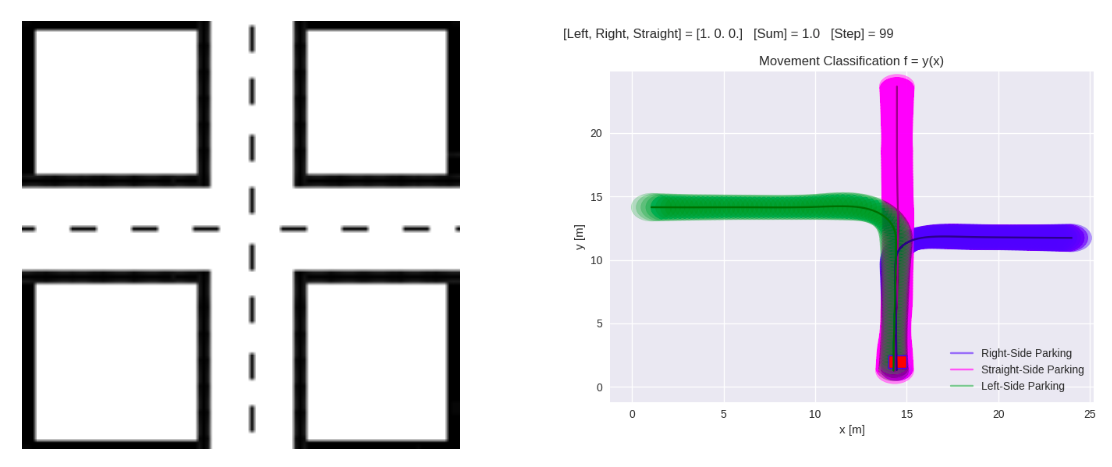
\includegraphics[width=13cm]{img/XInt.png}
	\caption{The left side of the figure shows how X-Intersection map, used for experiments, looks like. The right side of the figure shows the probabilistic prediction model, learned by algorithm:  blue, magenta and green areas show the mean trajectory and standard deviation for respectively \textcolor{blue}{right}, \textcolor{magenta}{straight} and \textcolor{green}{left} movement classes. The right side of the figure contains other important information: movement \textcolor{red}{start position} is $x_0,y_0 = (14.5, 2.0)$, illustrated with red rectangular and initial belief for each movement class with this setup is $b_0 = (0.333, 0.333, 0.333)$}
	\label{fig:Xint}    
\end{figure}

\subsubsection{Experiments Made Using X-Intersection. Movement Classification}

In the X intersection section, we have $3$ movement classes: right, straight and left, Figure~\ref{fig:MovClasses} illustrates trajectories with which experiments was made.

\begin{figure}[H]
	\centering  	
	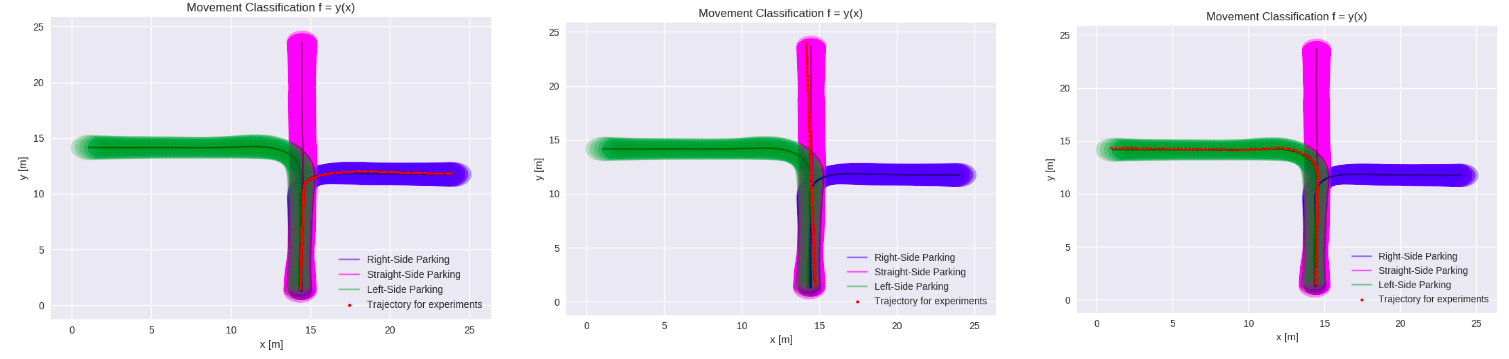
\includegraphics[width=18cm]{img/movetr.png}
	\caption{The figure shows, trajectories with which experiments were made. \textcolor{red}{Testing trajectories} are in red. The picture on the left shows a trajectory which classified as right, middle picture - as straight and the right picture as left movement class. Testing trajectories do not belong to the training data set}
	\label{fig:MovClasses}    
\end{figure}

As mentioned above in order to test algorithm we are using interpolated trajectories since all of them are not equal length/time-step wise. Due to method introduced in Chapter 3, Subsection 3.2, the  number of time steps can be chosen freely. In order to see if the number of time steps have any affect on results, we checked how much of trajectory need to be passes to the algorithm to get the correct prediction. Results of this experiment with movement to the right is in the table~\ref{table:CompareRight}:

\begin{table}[H]
	\centering
	\begin{tabular}{|c|c|c|c|c|c|c|c|c|c|c|c|} 
		\hline
		\multicolumn{12}{|c|}{Time Steps in Trajectories} \\
		\hline
		& $10$ & $20$ & $30$ & $40$ & $50$ & $60$ & $70$ & $80$ & $90$ & $100$ & $200$ \\ [0.5ex] 
		\hline\hline
		How many steps needed to go               & $4$ & $7$ & $11$ & $15$ & $20$ & $24$ & $28$ & $32$ & $38$ & $40$ & $80$ \\ [1ex]
		How much trajectory was needed to see, \% & $40$ & $35$ & $36.7$ & $37.5$ & $40$ & $40$ & $40$ & $40$ & $42.2$ & $40$ & $40$ \\ [1ex]
		\hline
	\end{tabular}
	\caption{Average time-steps needed to predict trajectory. The same trajectories were tested, just were interpolated differently. The second row, says after how many steps direction was recognized correctly (belief for going to that direction is >0.5 and after that step prediction for other directions do not occur). The third row shows how much trajectory needed to be seen to make a correct prediction. Trajectory direction is right}
	\label{table:CompareRight}
\end{table}

The table \ref{table:CompareStraight} summaries how prediction precision is affected by the number of time steps in trajectory while moving straight:

\begin{table}[H]
	\centering
	\begin{tabular}{|c|c|c|c|c|c|c|c|c|c|c|c|} 
		\hline
		\multicolumn{12}{|c|}{Time Steps in Trajectories} \\
		\hline
		& $10$ & $20$ & $30$ & $40$ & $50$ & $60$ & $70$ & $80$ & $90$ & $100$ & $200$ \\ [0.5ex] 
		\hline\hline
		How many steps needed to go               & $3$  & $6$  & $8$    & $11$   & $15$ & $18$ & $20$   & $23$    & $28$   & $30$ & $60$ \\ [1ex]
		How much trajectory was needed to see, \% & $30$ & $30$ & $26.7$ & $27.5$ & $30$ & $30$ & $28.6$ & $28.75$ & $31.1$ & $30$ & $30$ \\ [1ex]
		\hline
	\end{tabular}
	\caption{Average time-steps needed to predict trajectory. The same trajectories were tested, just were interpolated differently. The second row, says after how many steps direction was recognized correctly (belief for going to that direction is >0.5 and after that step prediction for other directions do not occur). The third row shows how much trajectory needed to be seen to make a correct prediction. Trajectory direction is straight}
	\label{table:CompareStraight}
\end{table}

The table~\ref{table:CompareLeft} summaries how prediction precision is affected by the number of time steps in trajectory, while moving to the left:

\begin{table}[H]
	\centering
	\begin{tabular}{|c|c|c|c|c|c|c|c|c|c|c|c|} 
		\hline
		\multicolumn{12}{|c|}{Time Steps in Trajectories} \\
		\hline
		& $10$ & $20$ & $30$ & $40$ & $50$ & $60$ & $70$ & $80$ & $90$ & $100$ & $200$ \\ [0.5ex] 
		\hline\hline
		How many steps needed to go               & $3$  & $7$  & $10$    & $14$ & $17$ & $20$  &  $23$   & $28$ & $30$   & $31$ & $60$ \\ [1ex]
		How much trajectory was needed to see, \% & $30$ & $35$ & $33.3$ & $35$  & $34$ & $33.3$ & $32.9$ & $35$  & $33.3$ & $31$ & $30$ \\ [1ex]
		\hline
	\end{tabular}
	\caption{Average time-steps needed to predict trajectory. The same trajectories were tested, just were interpolated differently. The second row, says after how many steps direction was recognized correctly (belief for going to that direction is >0.5 and after that step prediction for other directions do not occur). The third row shows how much trajectory needed to be seen to make a correct prediction. Trajectory direction is left}
	\label{table:CompareLeft}
\end{table}

From the results of tables~\ref{table:CompareRight}, ~\ref{table:CompareStraight} and ~\ref{table:CompareLeft}  we can see that our normalization method is working and number of times steps does not effect results so much. For the following experiments we choose to with $10$ and $100$ time steps.

\paragraph{Movement Classification: Right}

To illustrate how probabilistic intention prediction algorithm is working, we used pre-recorded trajectory, interpolated it to $10$ steps and made figure which illustrates prediction making results step-by-step.  

Figure~\ref{fig:rightPrediction} shows these results. From the series of plots, we can see that in the $5$th step algorithm beliefs that direction is right (result is equals to $1$). In the figure step number is $4$, because counting starts with $0$. Before $5$th steps algorithm was also thinking that a car can go straight, it happened because values of standard deviation for testing trajectory was very closer to straight class than right or left. After making the $5$th step algorithm knew for sure that movement direction is right since values for straight and left directions were very far away from the current car position. 

\begin{figure}[H]
	\centering  	
	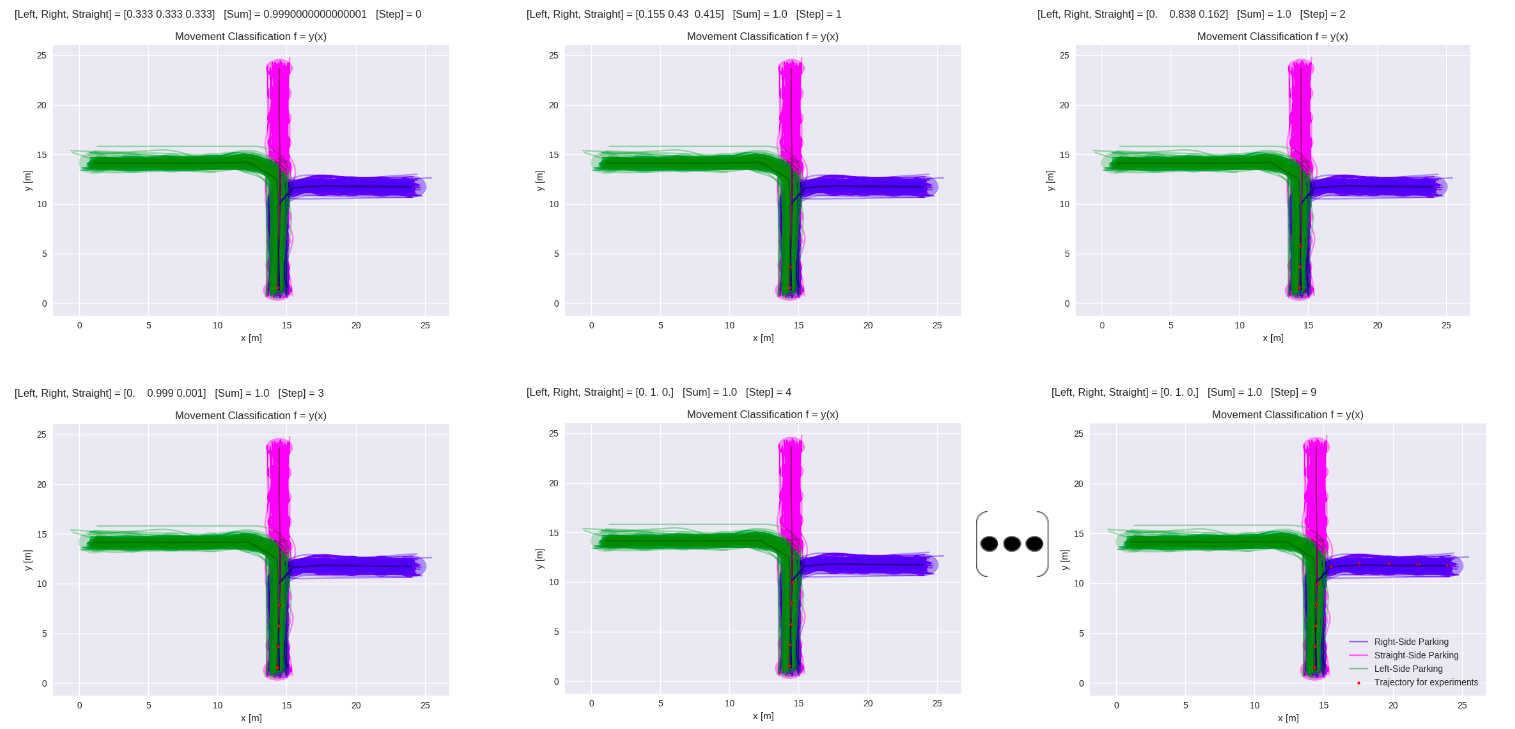
\includegraphics[width=18cm]{img/0_prediction_right.PNG}
	\caption{Process of prediction making for trajectory which belongs to the right movement class. Trajectory has $10$-time steps (counting from $0$ to $9$) and results after each time step are shown separately. After Step = $4$  prediction that movement is to the right is equal to $1.0$, due to that lack of space and the same result, we skipped to show step = $5$ - $8$}
	\label{fig:rightPrediction}    
\end{figure}

%To be able to see how beliefs are changing over time for the same just differently interpolated trajectory Figure~\ref{fig:CompareRight} was made. Left picture in the figure illustrates how belief changes when trajectory has $10$ points and when the same trajectory is interpolated $100$ times.

%\begin{figure}[H]
%	\centering  	
%	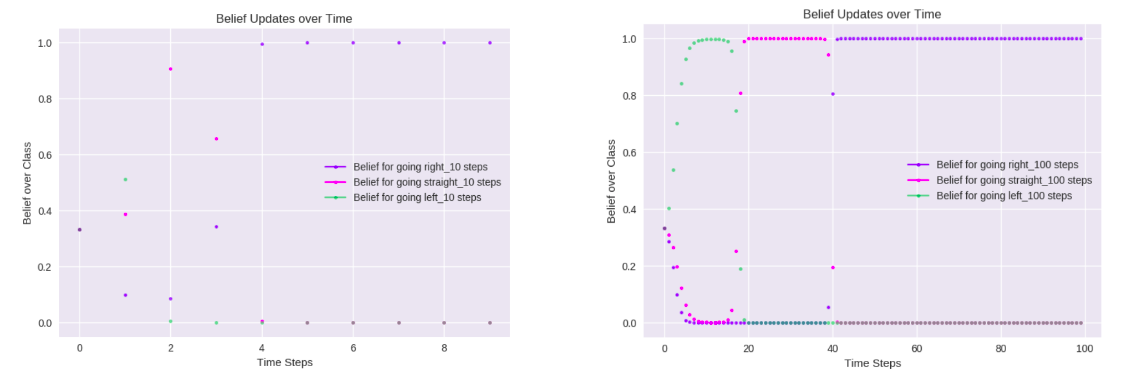
\includegraphics[width=13cm]{img/compare_right.png}
%	\caption{Belief changes over time. The same trajectory, just interpolated differently (for $10$ and for $100$-time steps). The left side of the figure illustrates belief changes for a trajectory with 10 steps and on the right side of the figure is trajectory with $100$ steps. Trajectory belong to right movement class}
%	\label{fig:CompareRight}    
%\end{figure}

While making experiments, there were a lot of trajectory tested. We noticed that even if trajectories belong to the same movement class, all of them are different (e.g. starting point slightly changes, some turnings are not so smooth as others, etc). All this results in being recognized correctly in a different time: "better" trajectories (e.g. the ones which are closer to the mean trajectory of movement class) are predicted correctly faster than the ones which are "worse" (e.g. making movement for one or another direction, not keeping straight line, etc.). To be able to see how belief changing over time for different trajectories and visually to see which trajectory is recognize faster than another Figure~\ref{fig:10Rights} was made. This figure was created just to show how fast (time step wise) trajectories are predicted correctly, figure does not show how each trajectory looks like. Figure~\ref{fig:10Rights} contains 10 random different trajectories of right movement class (which does not belong to training data set), interpolated for $100$-time steps each.

\begin{figure}[H]
	\centering  	
	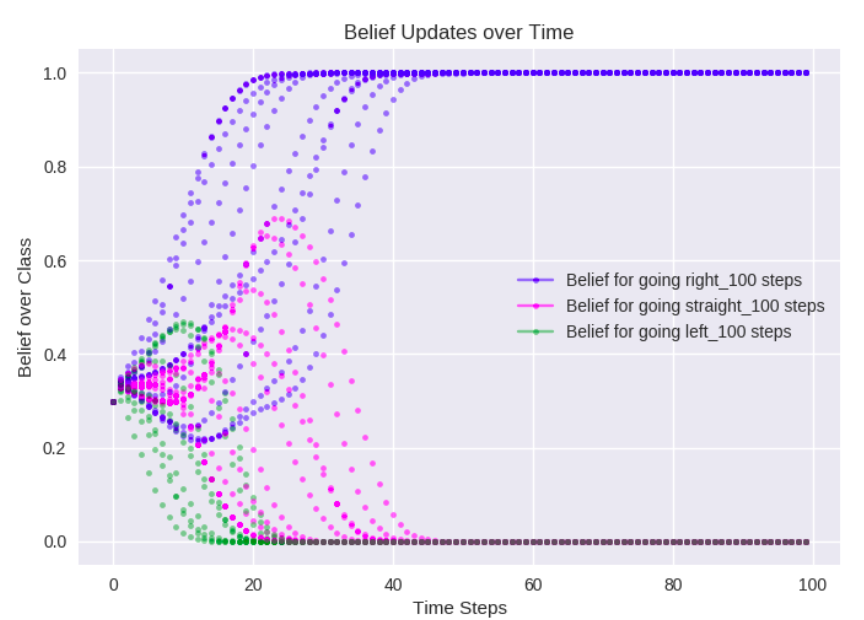
\includegraphics[width=7cm]{img/10right.png}
	\caption{Belief changes over time. $10$ random trajectories (which does not belong to training data set) were interpolated for $100$-time steps and tested with probabilistic intention prediction algorithm to see what is the pattern of for recognizing trajectories. Results shows that all trajectories were recognized correctly, just for some of them it took more time to be predict correctly. All tested trajectories belong to the same movement class. Movement class is right}
	\label{fig:10Rights}    
\end{figure}

Figure~\ref{fig:10Rights} illustrates that some trajectories required more time to be recognized correctly. As mentioned before, from this figure it is not possible to see and understand how \textit{the fastest} and \textit{the slowest} to recognize trajectories look like. For this purpose two more figures were computed: Figure~\ref{fig:RightGood} shows how \textit{the fastest} trajectory to recognize look like and how its belief changes over time and Figure~\ref{fig:RightBad} shows how \textit{the slowest} trajectory to recognize looks like.

\begin{figure}[H]
	\centering  	
	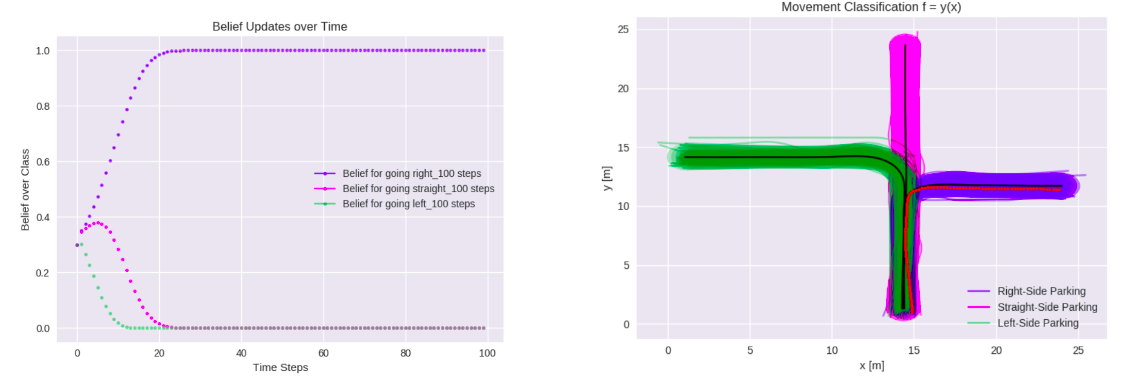
\includegraphics[width=13cm]{img/right_good.png}
	\caption{The fastest trajectory to recognize, taken from Figure~\ref{fig:10Rights}. On the left side of the figure belief changing over time is shown, from it is possible to see that trajectory is correctly recognized within $20$ steps (out of $100$). The right image shows how the fastest trajectory to recognize looks like. Trajectory direction is right}
	\label{fig:RightGood}    
\end{figure}

\begin{figure}[H]
	\centering  	
	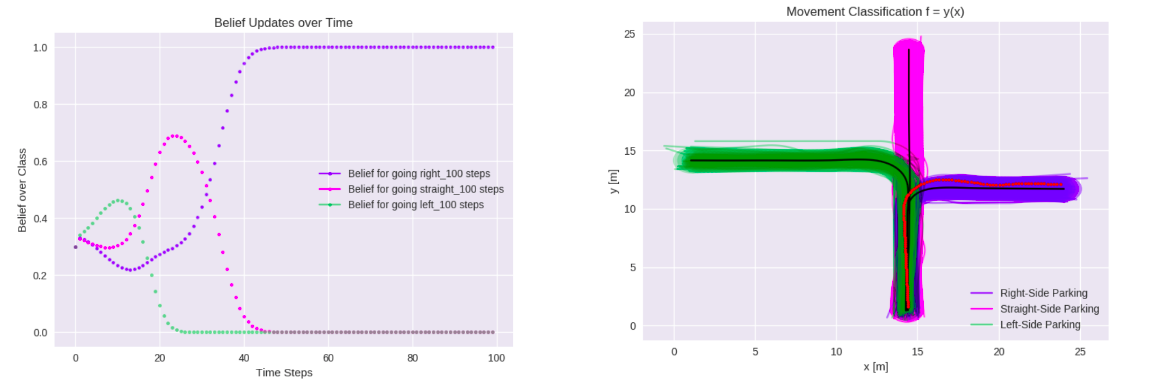
\includegraphics[width=13cm]{img/rightbad.png}
	\caption{The slowest trajectory to recognize, taken from Figure~\ref{fig:10Rights}. On the left side of the figure belief changing over time is shown, from it is possible to see that trajectory is correctly recognized within more than $40$ steps (out of $100$). The right image shows how the slowest trajectory to recognize looks like. Trajectory direction is right}
	\label{fig:RightBad}    
\end{figure}

As mentioned before \textit{the slowliness} in recognition can be explained by the position of the trajectory: it is close to all means, so it is natural that precise of prediction making can be disturbed in this case. \\
By looking at results from \textit{the fastest} trajectory to recognize, we can also make an assumption that trajectory is not on the all means, but it is closer to the standard deviation value of the right class and due to that precise of prediction making is better in this case. \\

\paragraph{Movement Classification: Straight}

Middle picture of Figure~\ref{fig:MovClasses} shows how straight movement class looks like. The table \ref{table:CompareStraight} shows the prediction preciseness depending on time steps in trajectory. As shown in a paragraph about the right movement class,  Figure~\ref{fig:straightPrediction} shows prediction making process, just this time for a straight movement class. From plots we can see that straight test trajectory is also easy to recognize: after $5$th step, a prediction that car is going straight is equal to $0.997$ and only growing while time passing. 

\begin{figure}[H]
	\centering  	
	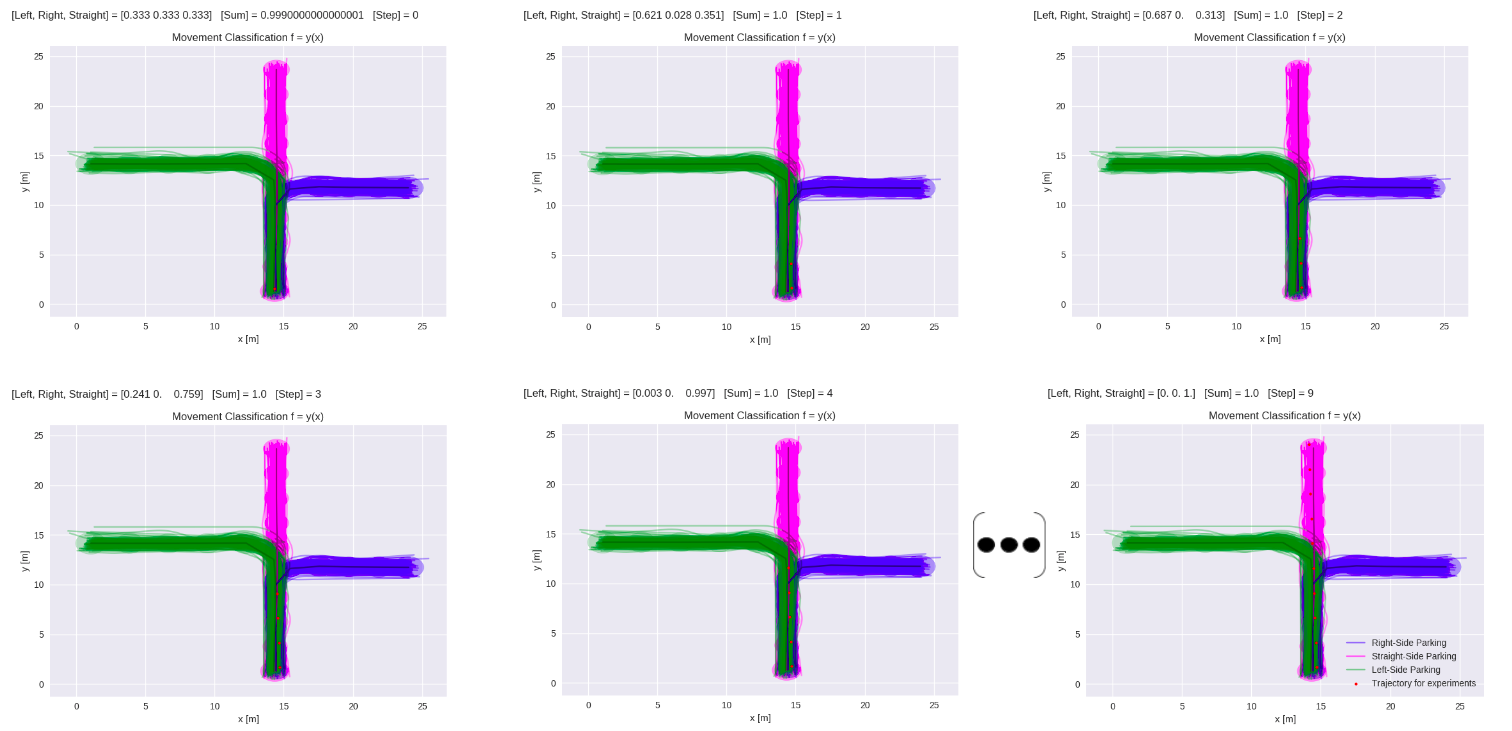
\includegraphics[width=17cm]{img/0_prediction_straight.PNG}
	\caption{Process of prediction making for trajectory which belongs to the straight movement class. Trajectory has $10$-time steps (counting from $0$ to $9$) and results after each time step are shown separately. After Step = $4$  prediction that movement is to straight is equal to $0.997$ and only getting bigger, due to that lack of space and the same result, we skipped to show step = $5$ - $8$}
	\label{fig:straightPrediction}    
\end{figure}

%As it was done with the right movement class Figure~\ref{fig:CompareStraight} shows the same trajectory, just interpolated for $10$ and $100$ time steps, and its belief changing over time.

%\begin{figure}[H]
%	\centering  	
%	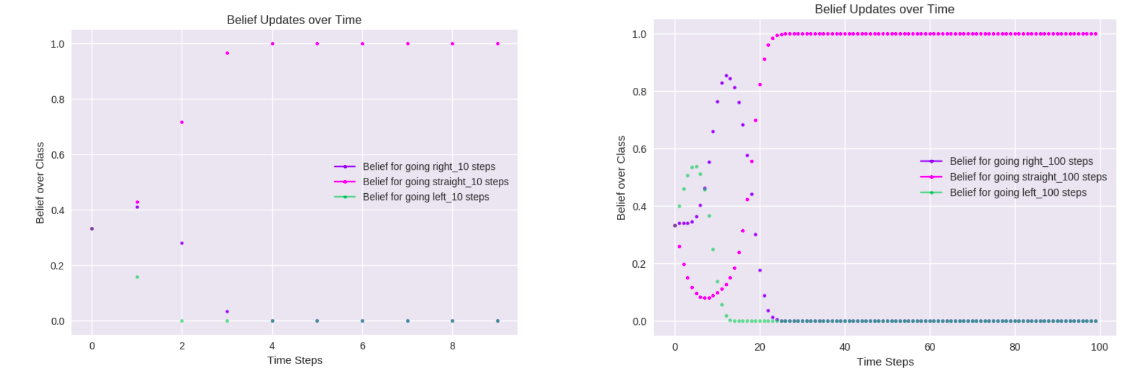
\includegraphics[width=13cm]{img/compare_straight.png}
%	\caption{Belief changes over time. The same trajectory, just interpolated differently (for $10$ and for $100$-time steps). The left side of the figure illustrates belief changes for a trajectory with 10 steps and on the right side of the figure is trajectory with $100$ steps. Trajectory belongs to straight movement class}
%	\label{fig:CompareStraight}    
%\end{figure}

Straight movement class also has different trajectories, and different time is needed to predict movement correctly. Figure~\ref{fig:10Straight} shows 10 random trajectories (which do not belong to algorithm training data set) and their belief updates over time. Figure~\ref{fig:StraightGood} and Figure~\ref{fig:StraightBad} respectively shows \textit{the fastest} and \textit{the slowest} trajectory to recognize. Trajectories were taken from the same set as in Figure~\ref{fig:10Straight}.

\begin{figure}[H]
	\centering  	 
	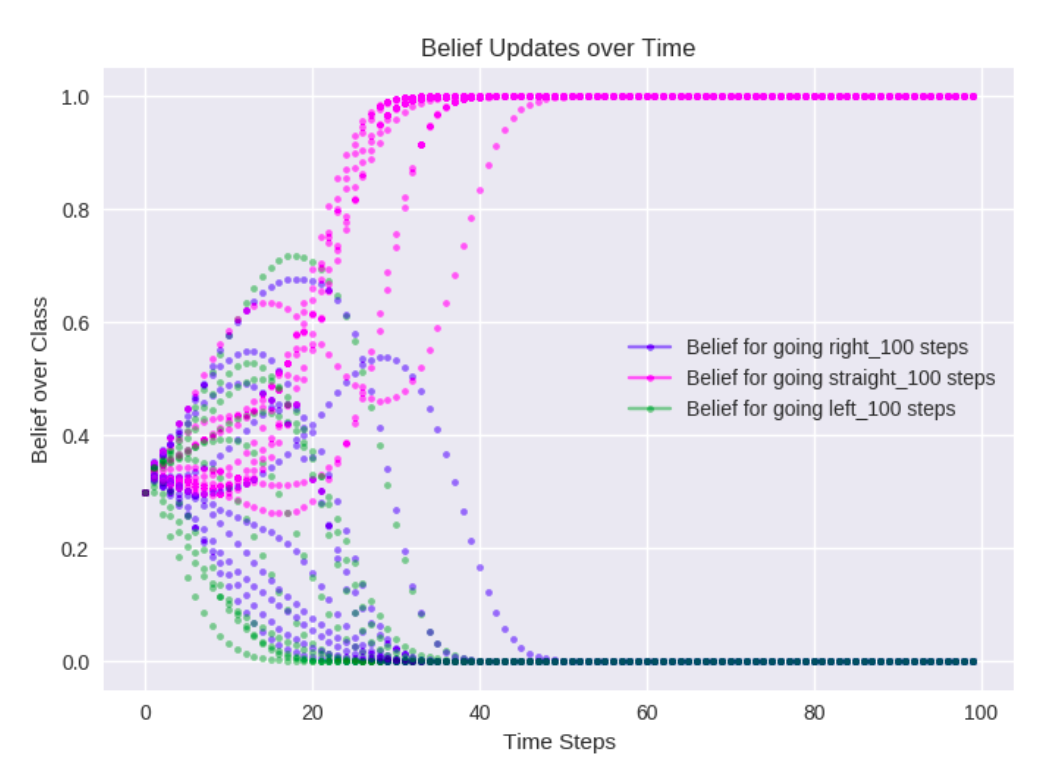
\includegraphics[width=6cm]{img/netstraight.png}
	\caption{Belief changes over time. $10$ random trajectories (which does not belong to training data set) were interpolated for $100$-time steps and tested with movement recognition algorithm to see which trajectory is predicted correctly faster and which slower. All tested trajectories belong to the same movement class. Movement class is straight}
	\label{fig:10Straight}    
\end{figure}

\begin{figure}[H]
	\centering  	
	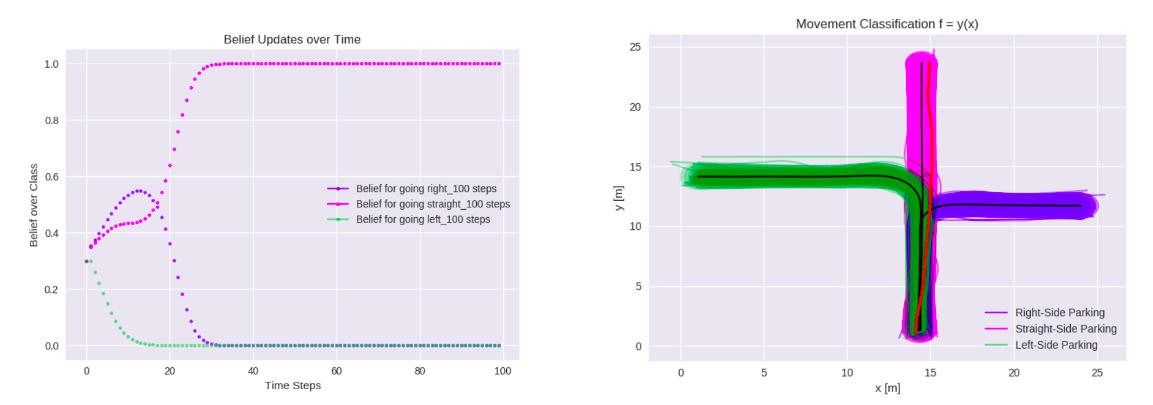
\includegraphics[width=13cm]{img/goodstr.png}
	\caption{The fastest trajectory to predict correctly, taken from Figure~\ref{fig:10Straight}. On the left side of the figure belief changing over time is shown, from it is possible to see that trajectory is correctly recognized within $30$ steps (out of $100$). The right image shows how the best trajectory looks like. Trajectory direction is straight}
	\label{fig:StraightGood}    
\end{figure}

\begin{figure}[H]
	\centering  	
	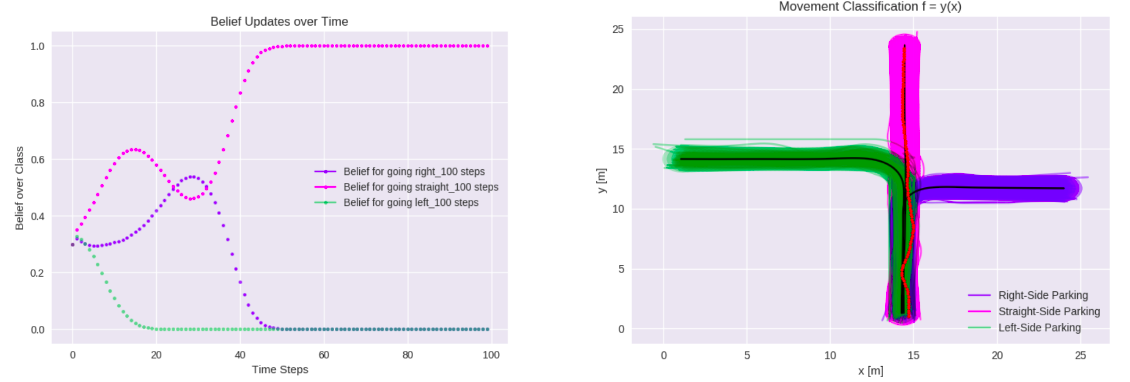
\includegraphics[width=13cm]{img/badstraight.png}
	\caption{The slowest trajectory to be predicted correctly, taken from Figure~\ref{fig:10Straight}. On the left side of the figure belief changing over time is shown, from it is possible to see that trajectory is correctly recognized within more than $50$ steps (out of $100$). The right image shows how the worse trajectory looks like. Trajectory direction is straight}
	\label{fig:StraightBad}    
\end{figure}

By looking at Figure~\ref{fig:StraightBad}, \textit{the long} time for being recognized and predicted correctly can be explained by the position of the trajectory: it is closer to standard deviation values of left class mean, this could be the case, why prediction is that car is going to the left, until it is sure that it is not going to the left for sure. \\
By looking at Figure~\ref{fig:StraightGood} \textit{the fastest} recognition can also be explain with assumption that trajectory and coordinates at each time step are closer to mean and it is in the range of standard deviation of the straight mean.

\paragraph{Movement Classification: Left}

Example of how left movement class looks like it is possible to find in the same Figure~\ref{fig:MovClasses} together with straight and right movement classes. The table \ref{table:CompareLeft} shows the prediction preciseness depending on time steps in trajectory. Figure~\ref{fig:leftPrediction} represents set of plots which represent prediction making process step by step. As usual test trajectory is interpolated to have $10$ time steps from results we can see that trajectory which belongs to the left movement class is very easily recognizable: after $3$rd step, a prediction that car is going straight is equal to $0.999$ and only growing while time passing. 

\begin{figure}[H]
	\centering  	
	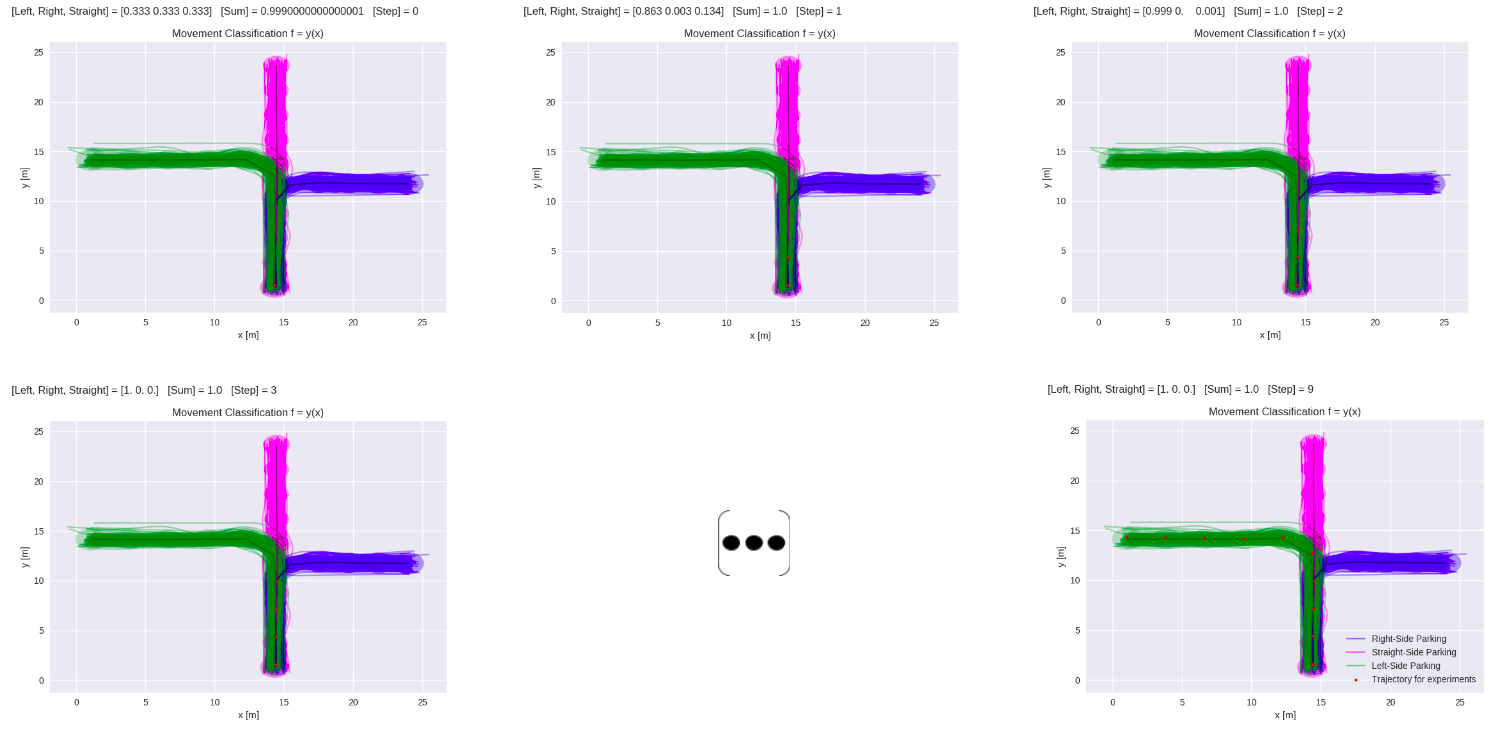
\includegraphics[width=16cm]{img/0_prediction_left.PNG}
	\caption{Process of prediction making for trajectory which belongs to the straight movement class. Trajectory has $10$-time steps (counting from $0$ to $9$) and results after each time step are shown separately. After Step = $2$  prediction that movement is to straight is equal to $0.999$ and only getting bigger, due to that lack of space and the same result, we skipped to show step = $4$ - $8$}
	\label{fig:leftPrediction}    
\end{figure}

%Following the same representation logic as in describing right and straight movement classes Figure~\ref{fig:CompareLeft} illustrates how beliefs are changing over time. Left graph of the Figure~\ref{fig:CompareLeft} shows belief changes when trajectory has $10$ points, a graph on the right, where is the same trajectory, just it was interpolated $100$ times.

%\begin{figure}[H]
%	\centering  	
%	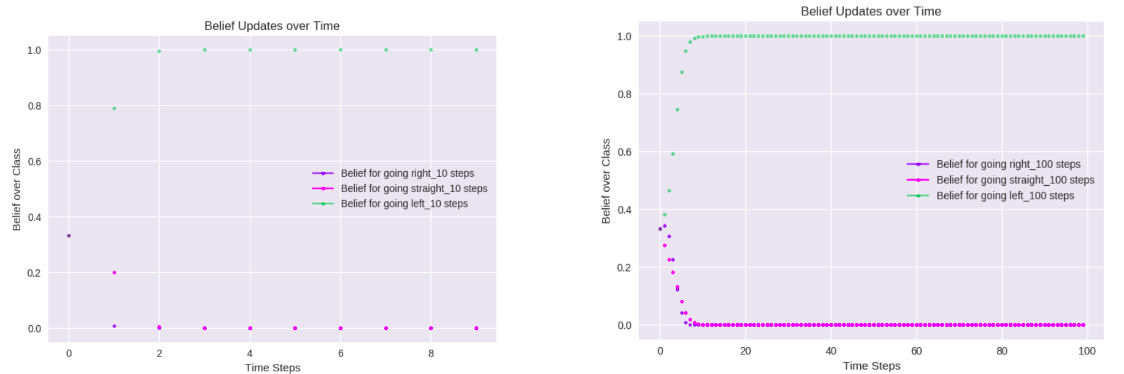
\includegraphics[width=13cm]{img/compareleft.png}
%	\caption{Belief changes over time. The same trajectory, just interpolated differently (for $10$ and for $100$-time steps). The left side of the figure illustrates belief changes for a trajectory with 10 steps and on the right side of the figure is trajectory with $100$ steps. Trajectory belongs to left movement class}
%	\label{fig:CompareLeft}    
%\end{figure}

Left movement class, as well as other movement classes, have trajectories which are predicted correctly not within the same amount of time steps. Figure~\ref{fig:10Left} shows $10$ random trajectories (which do not belong to algorithm training data set) and their belief updates over time. Figure~\ref{fig:LeftGood} and Figure~\ref{fig:LeftBad} respectively shows \textit{the fastest} and \textit{the slowest} trajectories to recognize, taken from the set of trajectories in Figure~\ref{fig:10Left}.

\begin{figure}[H]
	\centering  	
	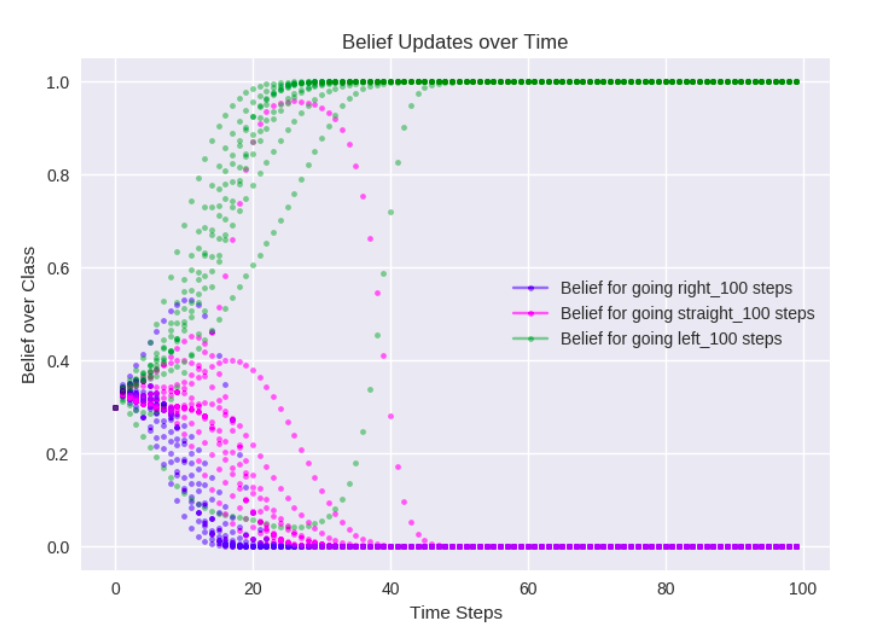
\includegraphics[width=7cm]{img/10left.png}
	\caption{Belief changes over time. $10$ random trajectories (which does not belong to training data set) were interpolated for $100$-time steps and tested with movement recognition algorithm to see which trajectory is easier recognized (better) and which one is more difficult (worse) to recognize correctly. All tested trajectories belong to the same movement class. Movement class is left}
	\label{fig:10Left}    
\end{figure}

\begin{figure}[H]
	\centering  	
	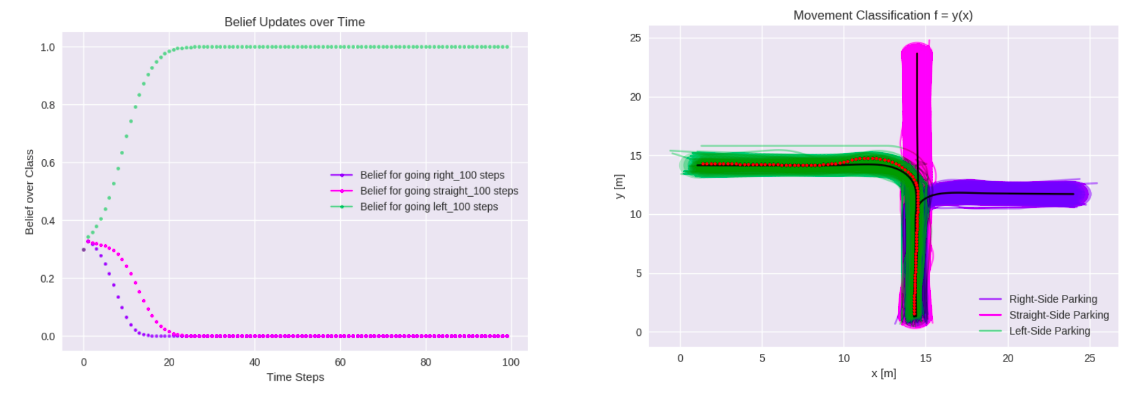
\includegraphics[width=13cm]{img/goodleft.png}
	\caption{The fastest recognizable trajectory, taken from Figure~\ref{fig:10Left}. On the left side of the figure belief changing over time is shown, from it is possible to see that trajectory is correctly recognized within the first $20$ steps (out of $100$). The right image shows how the best trajectory looks like. Trajectory direction is left}
	\label{fig:LeftGood}    
\end{figure}

\begin{figure}[H]
	\centering  	
	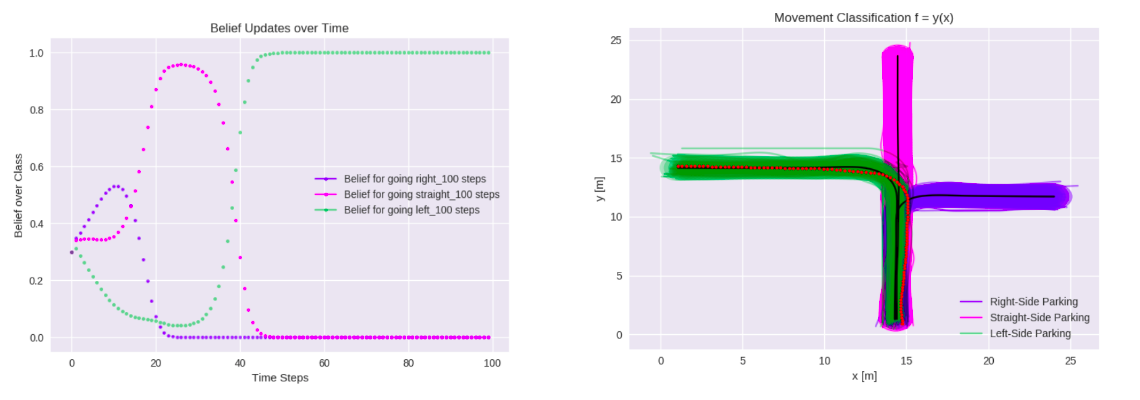
\includegraphics[width=12cm]{img/badleft.png}
	\caption{The slowest recognizable trajectory, taken from Figure~\ref{fig:10Left}. On the left side of the figure belief changing over time is shown, fromit is possible to see that trajectory is correctly recognized within more than $50$ steps (out of $100$). The right image shows how the worse trajectory looks like. Trajectory direction is left}
	\label{fig:LeftBad}    
\end{figure}

\subsection{Experiments Made Using T-Intersection}

As mentioned before we compute a probabilistic prediction model from demonstrations, depending on the map type probabilistic prediction model differs. T intersection has one direction less than X intersection, changes values of our model. Together with values which differs is initial belief $b_{0}$, for right movements class $b_{0} = 0.467$ and for left is equal to $b_{0} = 0.533$ (calculated using formulas from Chapter 3). The initial starting position is the same: $x_0,y_0 = (14.5, 2.0)$. Figure~\ref{fig:Tint} shows initial how tested map looks like and information which we have at the very beginning of the algorithm. 

\begin{figure}[H]
	\centering  	
	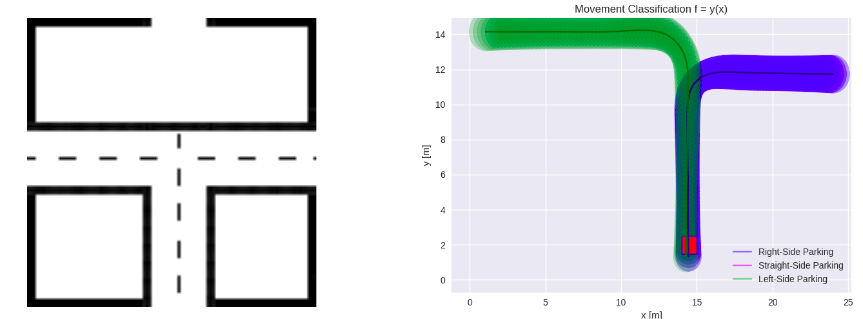
\includegraphics[width=11cm]{img/Tint.png}
	\caption{The left side of the figure shows how T-Intersection map, used for experiments, looks like. The right side of the figure shows the probabilistic prediction model, learned by algorithm:  blue and green areas show the mean trajectory and standard deviation for respectively \textcolor{blue}{right} and \textcolor{green}{left} movement classes. The right side of the figure contains other important information: movement \textcolor{red}{start position}  is $x_0,y_0 = (14.5, 2.0)$ and initial belief for each movement class, which is $b_0 \text{[left, right]}= (0.533, 0.467)$}
	\label{fig:Tint}    
\end{figure}

\subsubsection{Experiments Made Using T-Intersection. Movement Classification}

T intersection has $2$ movement classes: right and left, Figure~\ref{fig:MovClassesT} shows random testing trajectories (which do not belong to training data set) for each movement class.

\begin{figure}[H]
	\centering  	
	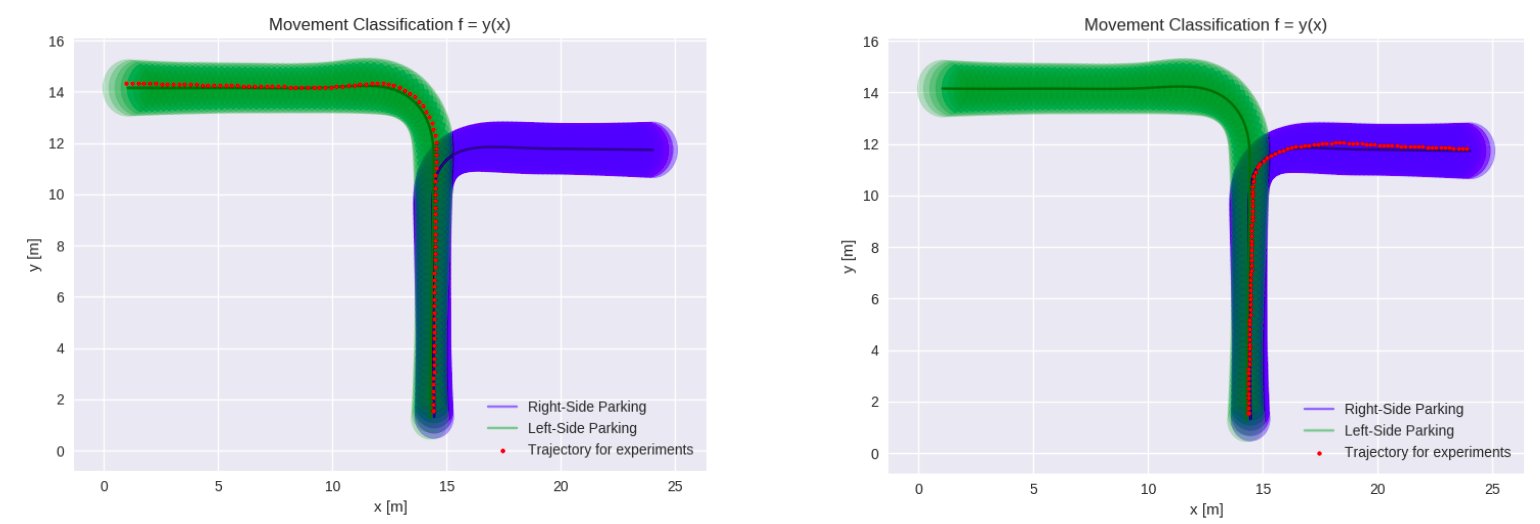
\includegraphics[width=13cm]{img/rightleftT.png}
	\caption{The figure shows random \textcolor{red}{testing trajectories} in red for each movement class. The picture on the left shows a trajectory from the right class and the right picture represents left movement class. Testing trajectories do not belong to the training data set}
	\label{fig:MovClassesT}    
\end{figure}

Precision of Prediction and dependence from time steps was tested with T intersection as well, results are in tables~\ref{table:CompareRightT} and ~\ref{table:CompareLeftT}.

\begin{table}[h!]
	\centering
	\begin{tabular}{|c|c|c|c|c|c|c|c|c|c|c|c|} 
		\hline
		\multicolumn{12}{|c|}{Time Steps in Trajectories} \\
		\hline
		& $10$ & $20$ & $30$ & $40$ & $50$ & $60$ & $70$ & $80$ & $90$ & $100$ & $200$ \\ [0.5ex] 
		\hline\hline
		How many steps needed to go               & $2$  & $4$  & $7$    & $10$ & $12$ & $15$  &  $16$   & $19$     & $22$   & $25$ & $40$ \\ [1ex]
		How much trajectory was needed to see, \% & $20$ & $20$ & $23.3$ & $25$  & $24$ & $25$ & $22.9$ & $23.75$  & $24.4$ & $25$ & $25$ \\ [1ex]
		\hline
	\end{tabular}
	\caption{Average time-steps needed to predict trajectory. The same trajectories were tested, just were interpolated differently. The second row, says after how many steps direction was recognized correctly (belief for going to that direction is >0.5 and after that step prediction for other directions do not occur). The third row shows how much trajectory needed to be seen to make a correct prediction. Trajectory direction is right}
	\label{table:CompareRightT}
\end{table}

\begin{table}[h!]
	\centering
	\begin{tabular}{|c|c|c|c|c|c|c|c|c|c|c|c|} 
		\hline
		\multicolumn{12}{|c|}{Time Steps in Trajectories} \\
		\hline
		& $10$ & $20$ & $30$ & $40$ & $50$ & $60$ & $70$ & $80$ & $90$ & $100$ & $200$ \\ [0.5ex] 
		\hline\hline
		How many steps needed to go               & $2$  & $4$  & $6$  & $9$     & $11$ & $13$  &  $15$   & $19$     & $19$   & $25$ & $50$ \\ [1ex]
		How much trajectory was needed to see, \% & $20$ & $20$ & $20$ & $22.5$  & $22$ & $21.7$ & $30$ & $23.75$  & $21.1$ & $25$ & $25$ \\ [1ex]
		\hline
	\end{tabular}
	\caption{Average time-steps needed to predict trajectory. The same trajectories were tested, just were interpolated differently. The second row, says after how many steps direction was recognized correctly (belief for going to that direction is >0.5 and after that step prediction for other directions do not occur). The third row shows how much trajectory needed to be seen to make a correct prediction. Trajectory direction is left}
	\label{table:CompareLeftT}
\end{table}

As in X intersection case we can see that our normalization method is working and number of times steps does not effect results so much. For the following experiments we choose to with $10$ and $100$ time steps. Following the same logic for result presentation as in X intersection is used.

\paragraph{Movement Classification: Right}

As just mentioned, an example of how the right movement class look like in T intersection environment is shown on the left side of Figure~\ref{fig:MovClassesT}. \\
This paragraph will provide the same figures just in different environmental set up as while working with X-intersection.

Table \ref{table:realStraight} shows prediction results of each step:

\begin{table}[h!]
	\centering
	\begin{tabular}{ |p{1.5cm}||p{1.5cm}|p{1.5cm}|p{1.5cm}|}
		\hline
		\multicolumn{4}{|c|}{Belief that Movement class is ...} \\
		\hline
		Time Step & Left & Right & Straight \\
		\hline
		0 & 0.524 & 0.476 & 0.0 \\
		1 & 0.284 & 0.716 & 0.0 \\
		2 & 0.010 & 0.980 & 0.0 \\
		3 - 9 & 0.0   & 1.0   & 0.0 \\
		\hline
	\end{tabular}
	\caption{Belief Update Over Time for straight trajectory. Algorithm knew to which direction car is going from the very beginning}
	\label{table:BelifRightT}
\end{table}

%As usual, Figure~\ref{fig:CompareRightT} shows how beliefs are changing over time for the same trajectory, just interpolated differently for $10$ (left side of the figure) and for $100$ (right side of the figure) time steps. 

%\begin{figure}[H]
%	\centering  	
%	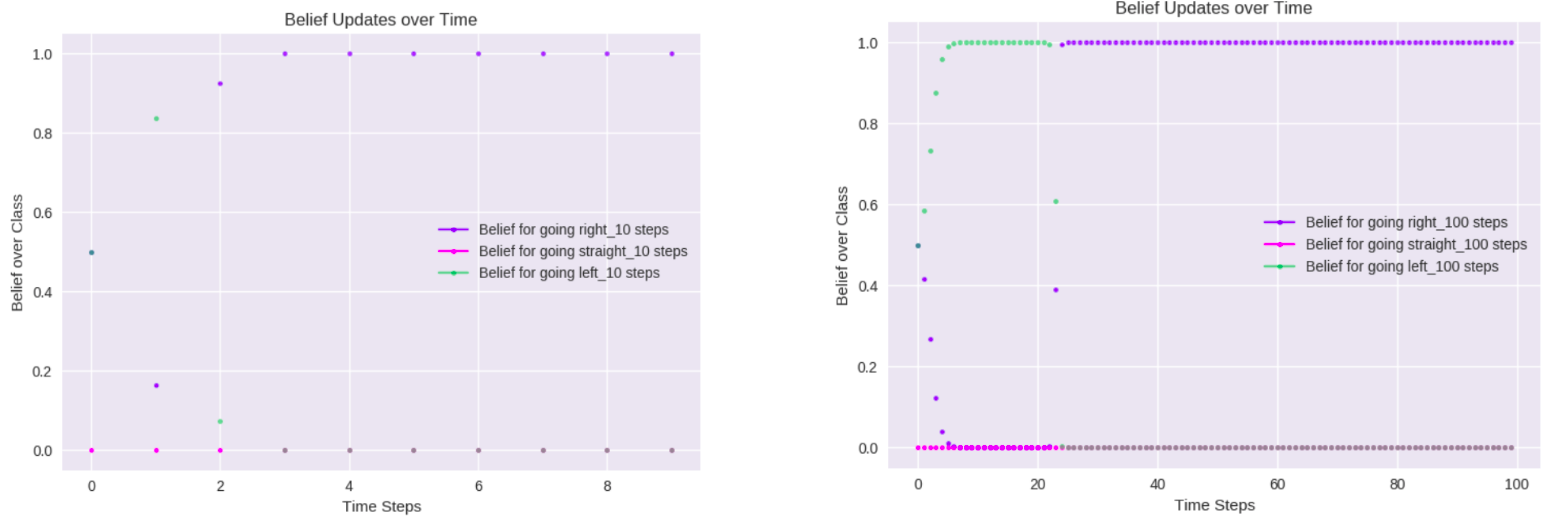
\includegraphics[width=13cm]{img/compareRightT.png}
%	\caption{Belief changes over time. The same trajectory, just interpolated differently (for $10$ and for $100$-time steps). The left side of the figure illustrates belief changes for a trajectory with 10 steps and on the right side of the figure is trajectory with $100$ steps. Trajectory belongs to right movement class}
%	\label{fig:CompareRightT}    
%\end{figure}

To be able to see how belief changing over times look for different trajectories and to differentiate which trajectories are \textit{faster} recognizable than another Figure~\ref{fig:10RightsT} was created. Here $10$ random trajectories (which do not belong to the training dataset) are plotted.

\begin{figure}[H]
	\centering  	
	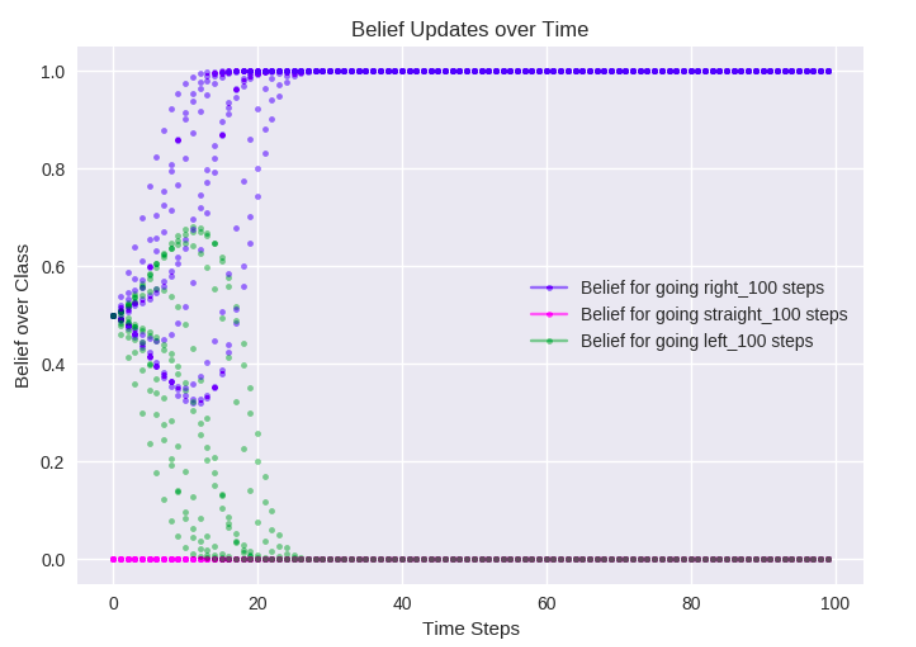
\includegraphics[width=8cm]{img/NetRightT.png}
	\caption{Belief changes over time. $10$ random trajectories (which does not belong to training data set) were interpolated for $100$-time steps and tested with movement recognition algorithm to see which trajectory is faster and which is slower recognizable. All tested trajectories belong to the same movement class. Movement class is right}
	\label{fig:10RightsT}    
\end{figure}

To see how \textit{the fastest} and \textit{the slowest} trajectories to recognize look like Figure~\ref{fig:RightGoodT} and Figure~\ref{fig:RightBadT} respectively were created.

\begin{figure}[H]
	\centering  	
	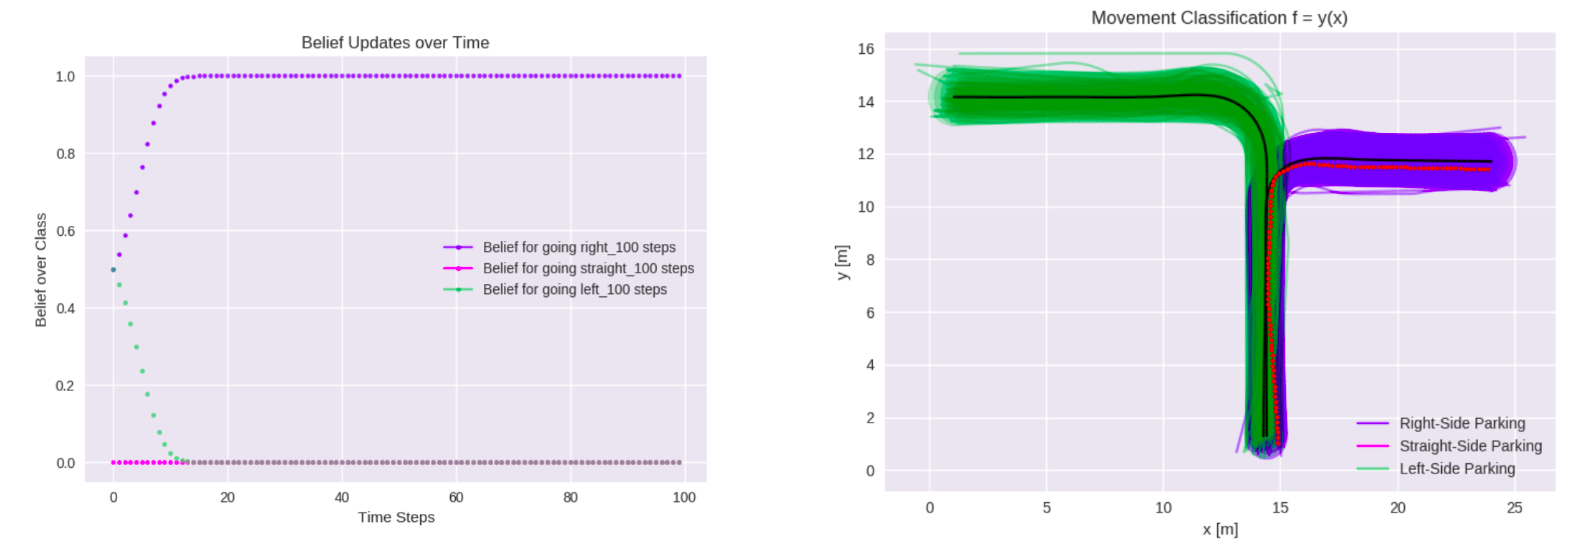
\includegraphics[width=14cm]{img/goodRightT.png}
	\caption{The fastest trajectory to recognize, taken from Figure~\ref{fig:10Left}. On the left side of the figure belief changing over time is shown, from it it is possible to see that trajectory is correctly recognized within the first $10$ steps (out of $100$). The right image shows how the best trajectory looks like. Trajectory direction is right}
	\label{fig:RightGoodT}    
\end{figure}

\begin{figure}[H]
	\centering  	
	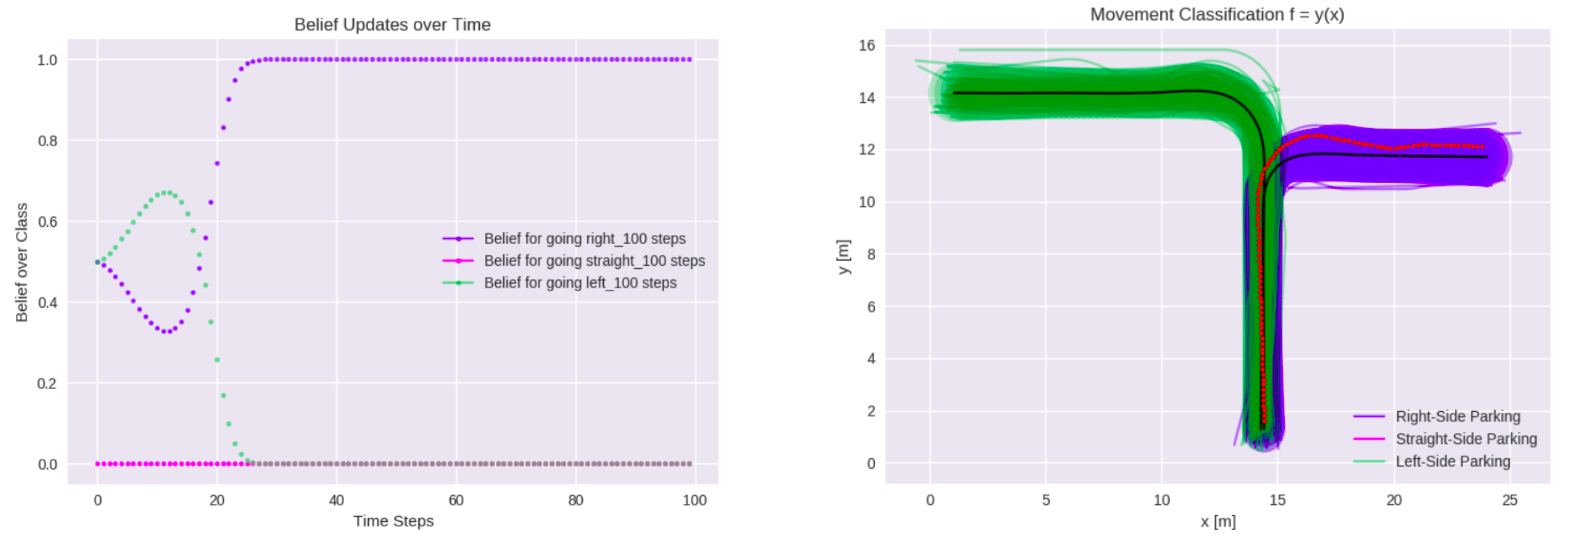
\includegraphics[width=14cm]{img/badRightT.png}
	\caption{The slowest trajectory in correct recognition, taken from Figure~\ref{fig:10Left}. On the left side of the figure belief changing over time is shown, from it it is possible to see that trajectory is correctly recognized within more than $30$ steps (out of $100$). The right image shows how the worse trajectory looks like. Trajectory direction is right}
	\label{fig:RightBadT}    
\end{figure}

From the Figure~\ref{fig:10RightsT} it is possible to see that correct prediction is made much faster than in case of an X-Intersection map (Figure~\ref{fig:10Rights}). This happened because of prior information and initial belief calculated according to it.

\paragraph{Movement Classification: Left}

An example of how the left movement class look like in T intersection environment is shown together with example of left movement class, just on the right side of Figure~\ref{fig:MovClassesT}. \\

Table \ref{table:BelifLEftT} shows prediction results of each step:

\begin{table}[h!]
	\centering
	\begin{tabular}{ |p{1.5cm}||p{1.5cm}|p{1.5cm}|p{1.5cm}|}
		\hline
		\multicolumn{4}{|c|}{Belief that Movement class is ...} \\
		\hline
		Time Step & Left & Right & Straight \\
		\hline
		0 & 0.524 & 0.476 & 0.0 \\
		1 & 0.997 & 0.003 & 0.0 \\
		2 - 9 & 1.0   & 0.0   & 0.0 \\
		\hline
	\end{tabular}
	\caption{Belief Update Over Time for straight trajectory. Algorithm knew to which direction car is going from the very beginning}
	\label{table:BelifLEftT}
\end{table}

%As usual, Figure~\ref{fig:CompareLeftT} shows how beliefs are changing over time for the same trajectory, just interpolated differently for $10$ (left side of the figure) and for $100$ (right side of the figure) time steps. 

%\begin{figure}[H]
%	\centering  	
%	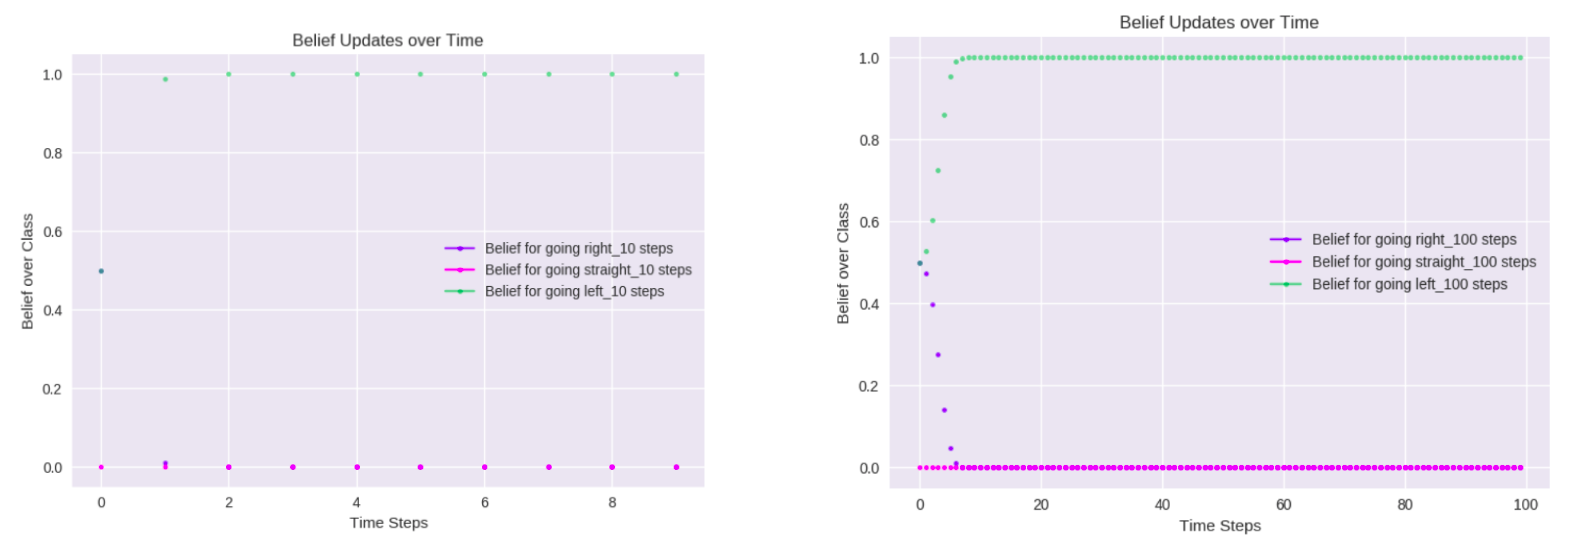
\includegraphics[width=13cm]{img/compareLeftT.png}
%	\caption{Belief changes over time. The same trajectory, just interpolated differently (for $10$ and for $100$-time steps). The left side of the figure illustrates belief changes for a trajectory with 10 steps and on the right side of the figure is trajectory with $100$ steps. Trajectory belongs to left movement class}
%	\label{fig:CompareLeftT}    
%\end{figure}

To be able to see how beliefs are changing over time withing different trajectories and compare how the movement recognition process looks we plotted 10 random trajectories going to the right. Results are shown in Figure~\ref{fig:10LeftsT}.

\begin{figure}[H]
	\centering  	
	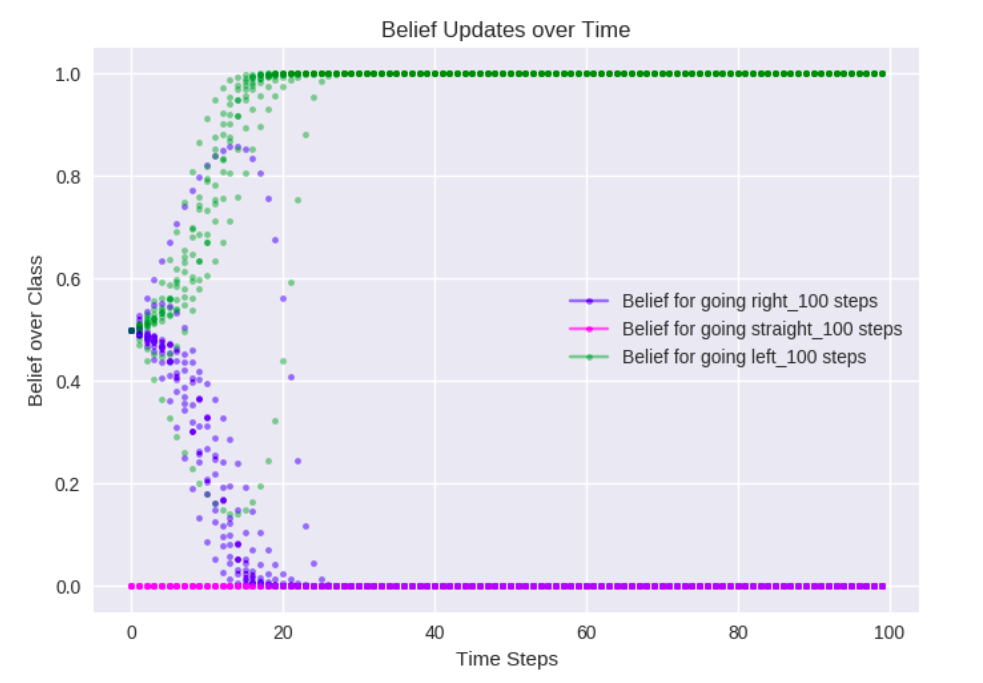
\includegraphics[width=7cm]{img/netLeftT.png}
	\caption{Belief changes over time. $10$ random trajectories (which does not belong to training data set) were interpolated for $100$-time steps and tested with movement recognition algorithm to see which trajectory is faster and which is slower recognizable. All tested trajectories belong to the same movement class. Movement class is left}
	\label{fig:10LeftsT}    
\end{figure}

Figure~\ref{fig:LeftGoodT} and Figure~\ref{fig:LeftBadT} show how \textit{the fastest} and \textit{the slowest}, respectively, trajectories to recognize look like 

\begin{figure}[H]
	\centering  	
	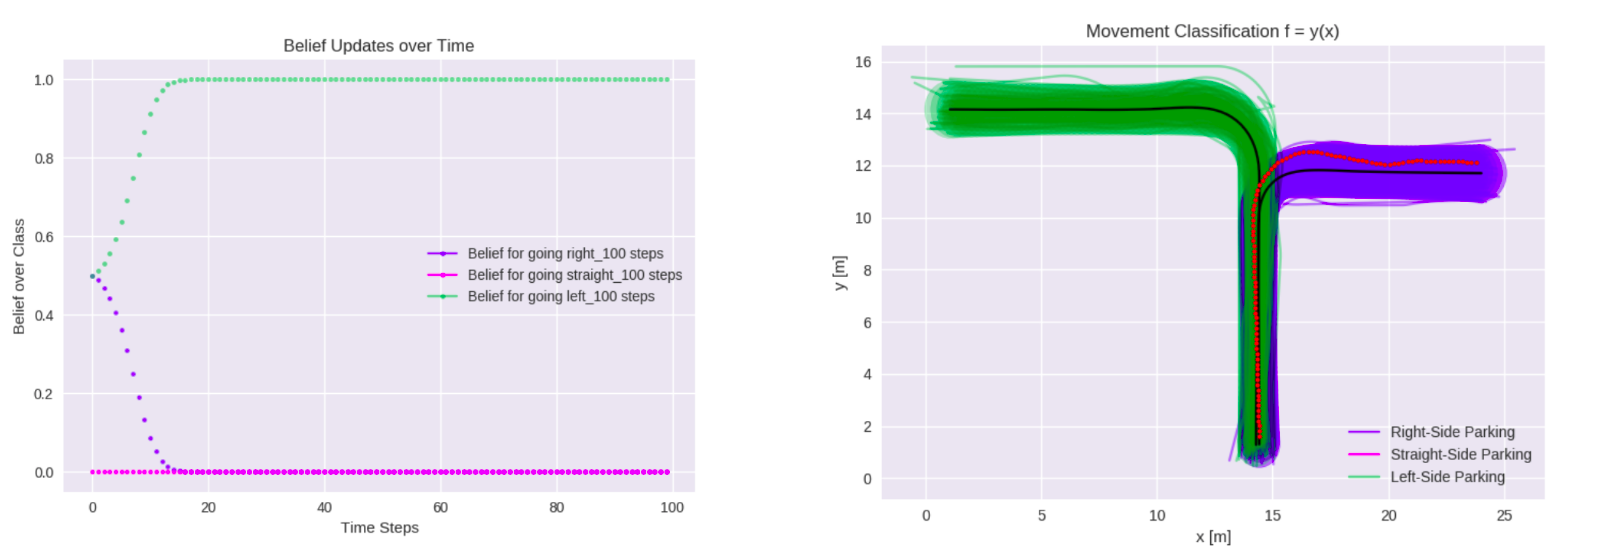
\includegraphics[width=13cm]{img/goodLeftT.png}
	\caption{The fastest trajectory to recognize, taken from Figure~\ref{fig:10Left}. On the left side of the figure belief changing over time is shown, from it it is possible to see that trajectory is correctly recognized within the first $20$ steps (out of $100$). The right image shows how the best trajectory looks like. Trajectory direction is left}
	\label{fig:LeftGoodT}    
\end{figure}

\begin{figure}[H]
	\centering  	
	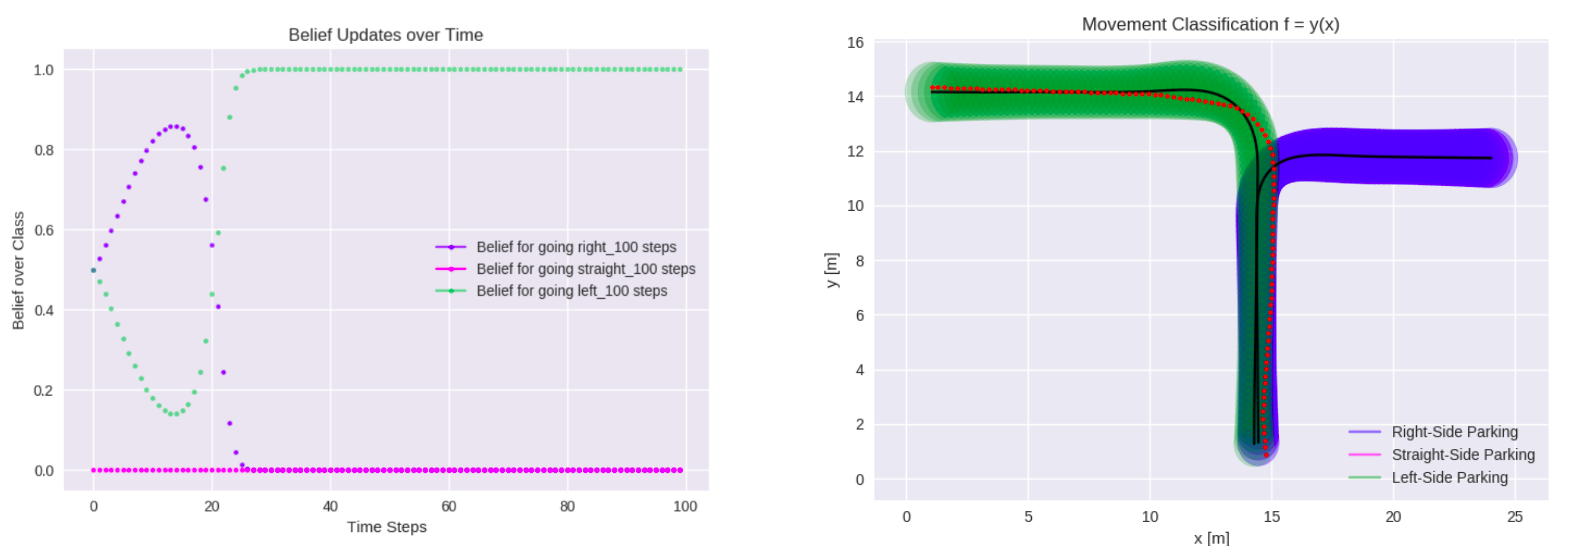
\includegraphics[width=13cm]{img/badleftT.png}
	\caption{The slowest trajectory to recognize, taken from Figure~\ref{fig:10Left}. On the left side of the figure belief changing over time is shown, from it it is possible to see that trajectory is correctly recognized within more than $30$ steps (out of $100$). The right image shows how the worse trajectory looks like. Trajectory direction is left}
	\label{fig:LeftBadT}    
\end{figure}

\subsubsection{Experiments Using Pre-Recorded Data. Comparison of Results in Different Environments}

Summarizing all results, described before, we can state that all trajectories are recognized and predicted correctly. Due to the shape and "smoothness" of trajectory one trajectories are recognized faster than another but after comparing the average number of points for differently interpolated trajectories we can say, that independently from the number of points in the trajectory and from direction class around $40$\% of trajectory needed to be seen to recognize trajectory correctly. A summary of X and T intersections are respectively in the table \ref{table:averageX} and \ref{table:avertageT}

\begin{table}[h!]
	\centering
	\begin{tabular}{ |c|c|c|c|}
		\hline
		\multicolumn{4}{|c|}{Movement Class} \\
		\hline
		& Right & Straight & Left \\
		\hline
		How much trajectory was needed to see & about $40$\% & about $20$\% & about $33$\% \\
		\hline
	\end{tabular}
	\caption{Average length of trajectory needed to predict movement class correctly in X intersection}
	\label{table:averageX}
\end{table}

\begin{table}[h!]
	\centering
	\begin{tabular}{ |c|c|c|}
		\hline
		\multicolumn{3}{|c|}{Movement Class} \\
		\hline
		& Right & Left \\
		\hline
		How much trajectory was needed to see & about $20$\% & about $25$\% \\
		\hline
	\end{tabular}
	\caption{Average length of trajectory needed to predict movement class correctly in T intersection}
	\label{table:avertageT}
\end{table}

Prediction is faster in T intersection because of the initial belief $b_{0}$, which belong to probabilistic prediction model learned from demonstrations, while in X intersection assumption about initial belief was that it is an equal possibility that car will go to any possible direction.

Below in the tables \ref{table:EdgeValuesX} and \ref{table:EdgeValuesT}  of the maximum, average and minimum length of trajectory, which was necessary for correct movement direction prediction. 

\begin{table}[h!]
	\centering
	\begin{tabular}{|c|c|c|c|c|c|c|c|c|}
		\hline
		\multicolumn{9}{|c|}{Movement Class} \\
		\hline
		\multicolumn{3}{|c|}{Right} & \multicolumn{3}{c}{Straight} & \multicolumn{3}{|c|}{Left}\\
		\hline
		Max Len. & Avg. Len. & Min Len. & Max Len. & Avg. Len. & Min Len. & Max Len. & Avg. Len. & Min Len. \\
		\hline
		$50$\% & about $40$\% & $25$\% & $40$\% & about $30$\% & $10$\% & $42$\% & about $33$\% & $15$\% \\
		\hline
	\end{tabular}
	\caption{Maximum, average and minimum length of trajectory needed to predict movement class correctly in X intersection per each movement class}
	\label{table:EdgeValuesX}
\end{table}

\begin{table}[h!]
	\centering
	\begin{tabular}{|c|c|c|c|c|c|}
		\hline
		\multicolumn{6}{|c|}{Movement Class} \\
		\hline
		\multicolumn{3}{|c}{Right} &  \multicolumn{3}{|c|}{Left}\\
		\hline
		Max Len. & Avg. Len. & Min Len. & Max Len. & Avg. Len. & Min Len. \\
		\hline
		$25$\% & about $15$\% & $25$\% & $30$\% & about $25$\% & $8$\% \\
		\hline
	\end{tabular}
	\caption{Maximum, average and minimum length of trajectory needed to predict movement class correctly in T intersection per each movement class}
	\label{table:EdgeValuesT}
\end{table}

\subsection{Trajectory Scaling}

As we noticed from results before the pattern of recognizing movement for the trajectory is similar when trajectory has $10$ and $100$ time steps. But for obvious reasons making a prediction for a trajectory with $100$ time steps is more precise, since it is doing more updates, but at the same time to make a prediction for trajectory with $100$ time steps is more difficult computation-wise, since calculations need to be done $10$ times more (and faster) in order to keep a prediction pace while car is moving. To solve this problem we asked ourselfs is it possible to get a prediction precision of $100$ time steps while making calculations only 10 times? \\
To make this possible into our prediction making algorithm we included scaling function, which is described before and in Figure~\ref{fig:PseudoScalling} it is possible to see the pseudo code for this process. To show the difference between scaled results and not scaled results two different graphs will be shown for one test.

\subsubsection{Trajectory Scaling. X-Intersection. Movement Classes}

 X-Intersection has $3$ different movement directions and figures below show the trajectory prediction for all $3$ classes before and after scaling.

\begin{figure}[H]
	\centering  	
	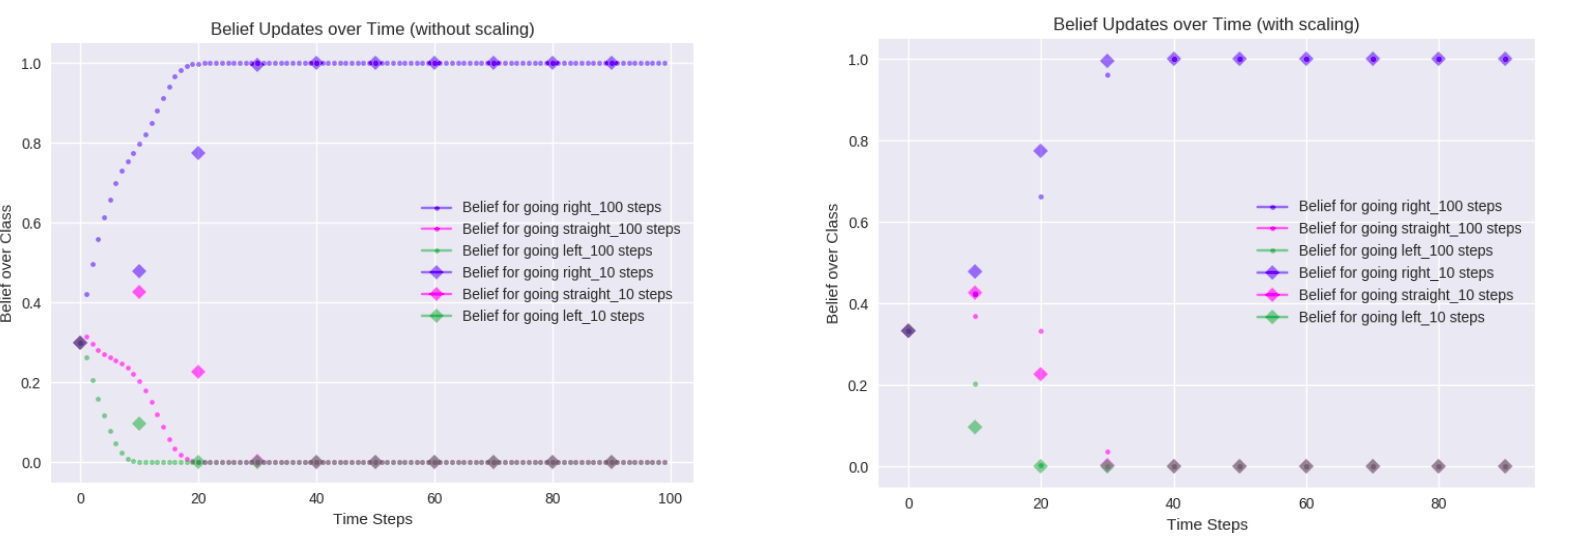
\includegraphics[width=13cm]{img/ScalingRightX.png}
	\caption{Belief updates over time. The picture on the left side of the figure shows the original belief update for the same trajectory interpolated for $10$ and $100$ time steps. The right side of the figure shows the prediction making process including scaling for the same trajectory interpolated for $10$ and $100$ time steps. For better visibility from trajectory with $100$ time steps was printed only $10$ points, matching points in from trajectory with  $10$ time steps. Trajectory direction is right}
	\label{fig:ScallingRightX}    
\end{figure}

\begin{figure}[H]
	\centering  	
	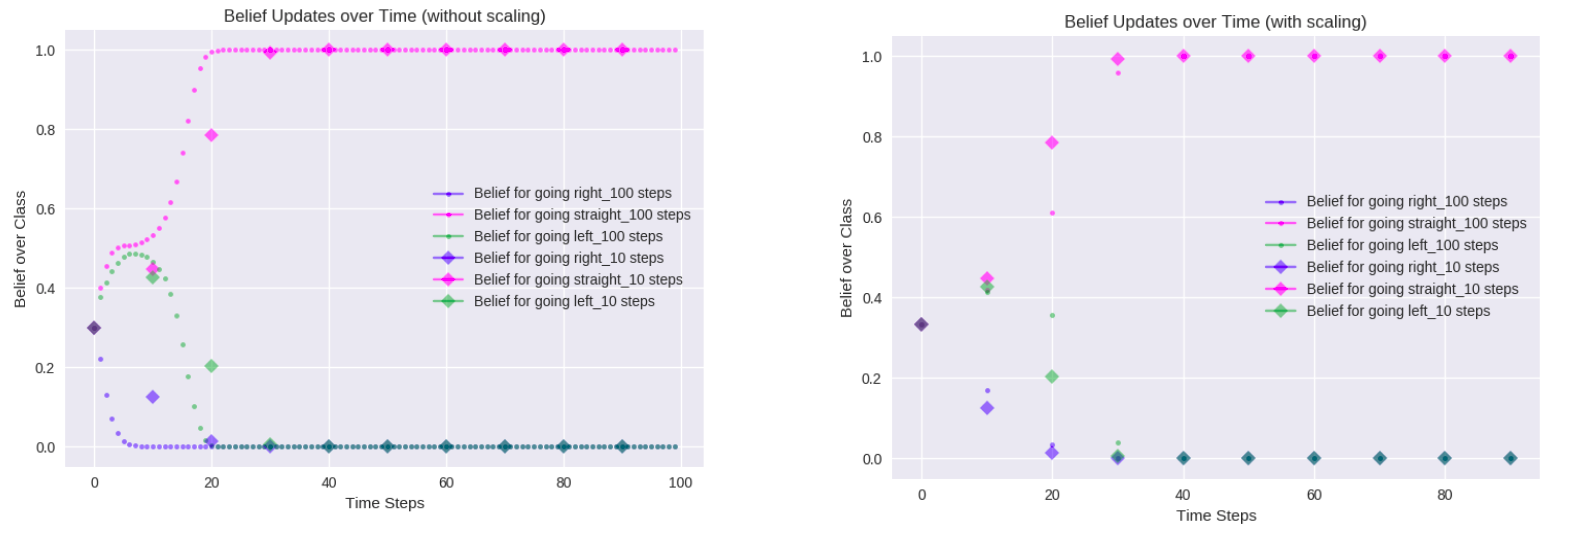
\includegraphics[width=13cm]{img/ScalingStraightX.png}
	\caption{Belief updates over time. The picture on the left side of the figure shows the original belief update for the same trajectory interpolated for $10$ and $100$ time steps. The right side of the figure shows the prediction making process including scaling for the same trajectory interpolated for $10$ and $100$ time steps. For better visibility from trajectory with $100$ time steps was printed only $10$ points, matching points in from trajectory with  $10$ time steps. Trajectory direction is straight}
	\label{fig:ScallingStraightX}    
\end{figure}

\begin{figure}[H]
	\centering  	
	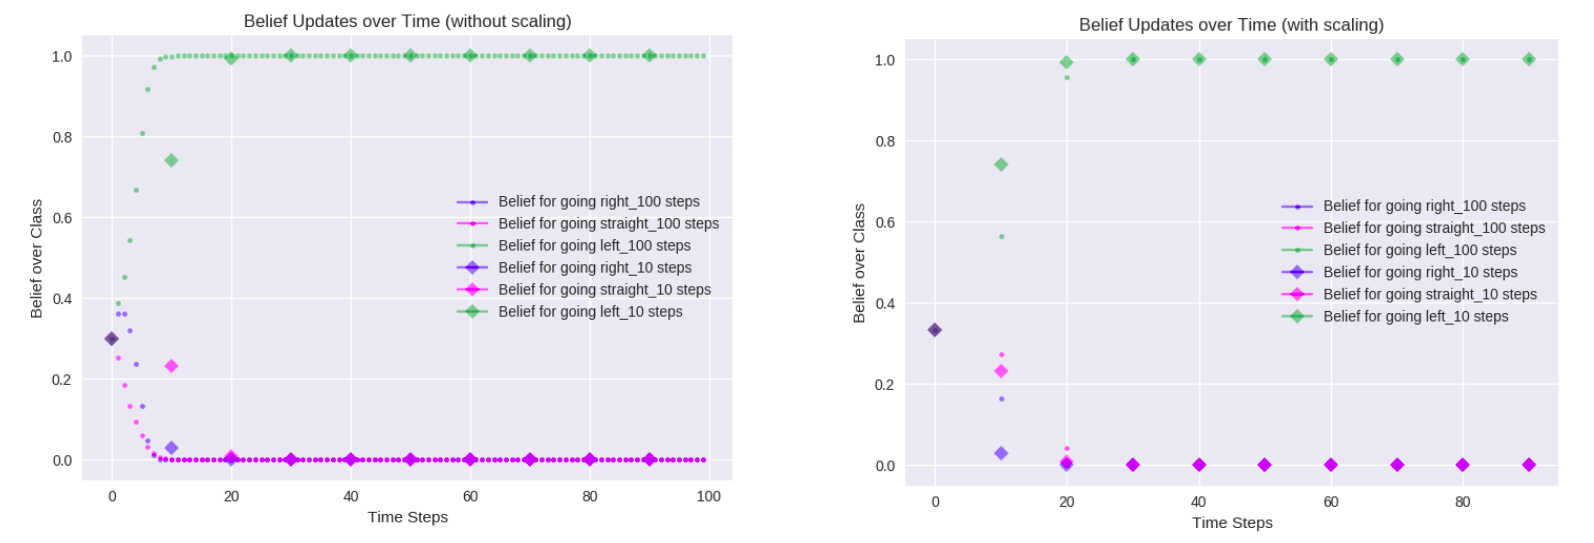
\includegraphics[width=13cm]{img/ScalingLeftX.png}
	\caption{Belief updates over time. The picture on the left side of the figure shows the original belief update for the same trajectory interpolated for $10$ and $100$ time steps. The right side of the figure shows the prediction making process including scaling for the same trajectory interpolated for $10$ and $100$ time steps. For better visibility from trajectory with $100$ time steps was printed only $10$ points, matching points in from trajectory with  $10$ time steps. Trajectory direction is left}
	\label{fig:ScallingLeftX}    
\end{figure}

\subsubsection{Trajectory Scaling. T-Intersection. Movement Classes}

T-Intersection has $2$ different movement directions: right and left. Figures below show the trajectory prediction for all classes before and after scaling.

\begin{figure}[H]
	\centering  	
	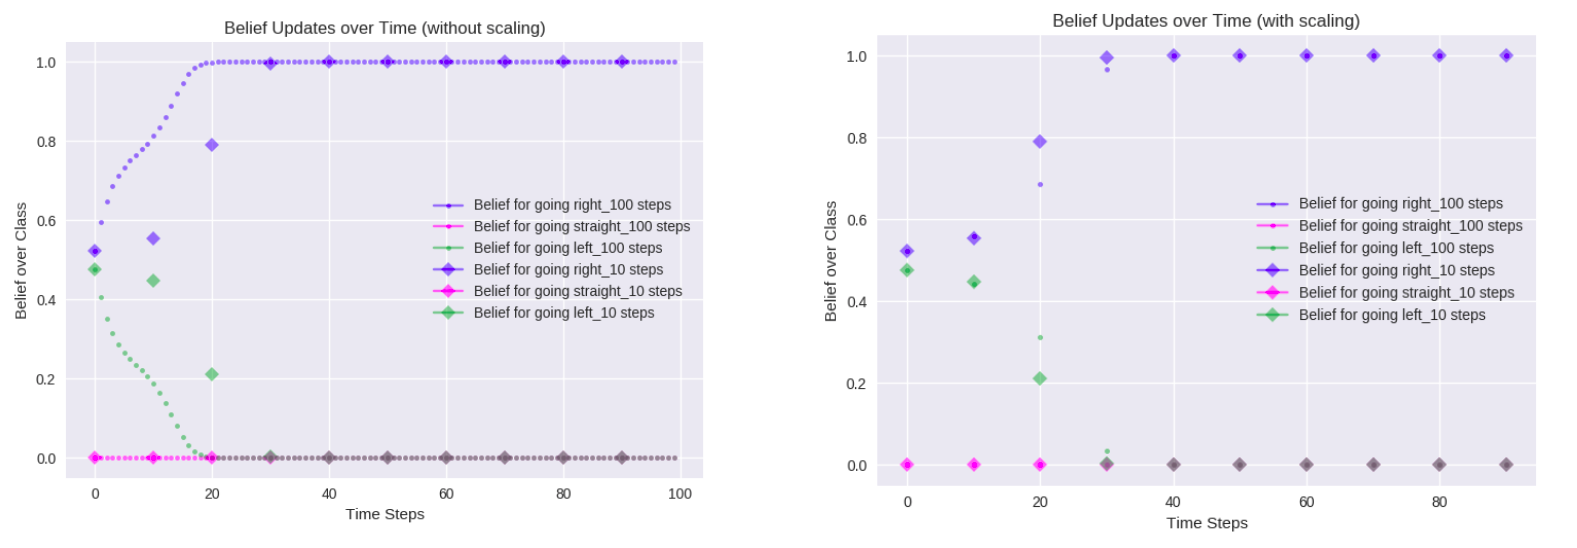
\includegraphics[width=13cm]{img/ScalingRightT.png}
	\caption{Belief updates over time. The picture on the left side of the figure shows the original belief update for the same trajectory interpolated for $10$ and $100$ time steps. The right side of the figure shows the prediction making process including scaling for the same trajectory interpolated for $10$ and $100$ time steps. For better visibility from trajectory with $100$ time steps was printed only $10$ points, matching points in from trajectory with  $10$ time steps. Trajectory direction is right}
	\label{fig:ScallingRightT}    
\end{figure}

\begin{figure}[H]
	\centering  	
	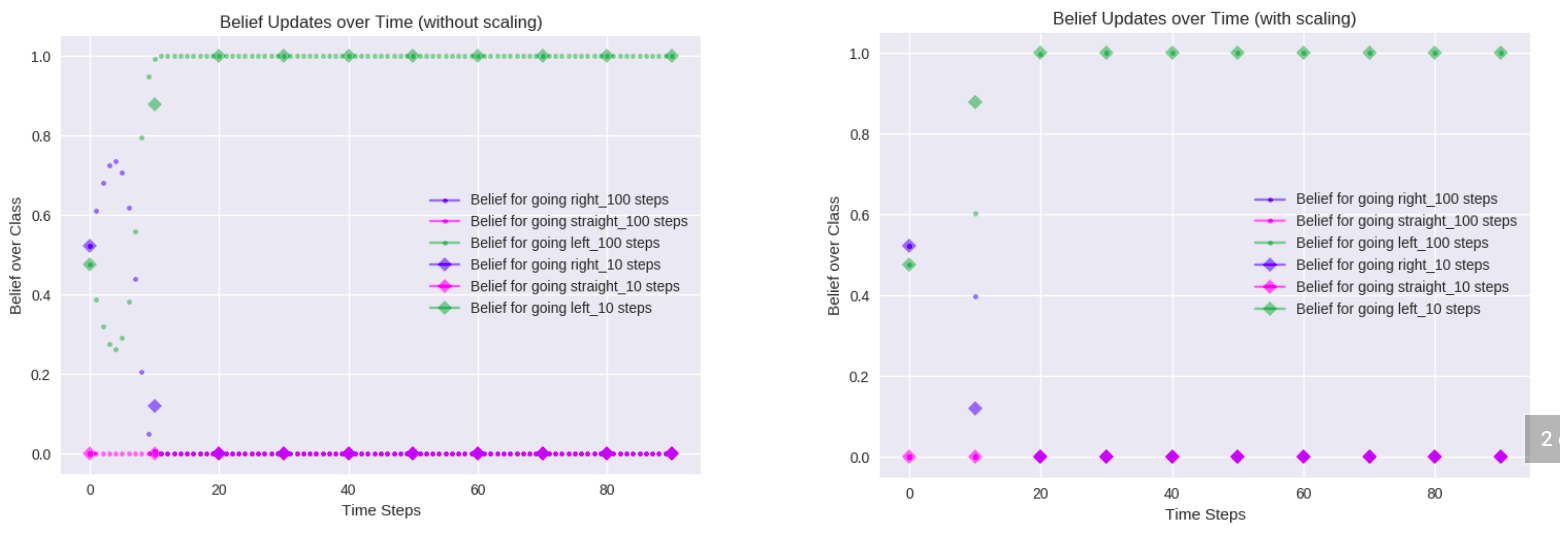
\includegraphics[width=13cm]{img/ScalingLeftT.png}
	\caption{Belief updates over time. The picture on the left side of the figure shows the original belief update for the same trajectory interpolated for $10$ and $100$ time steps. The right side of the figure shows the prediction making process including scaling for the same trajectory interpolated for $10$ and $100$ time steps. For better visibility from trajectory with $100$ time steps was printed only $10$ points, matching points in from trajectory with  $10$ time steps. Trajectory direction is left}
	\label{fig:ScallingLeftT}    
\end{figure}

From the results for X and T intersections, we can see that the process of scaling is working and it gives much closer results between differently interpolated trajectories. Scaling can be used when for some reasons it is not possible to compute predictions as often. But for critical situations we still suggest to used not scaled method and use trajectory interpolated for more time steps.

\subsection{Full Trajectory Prediction, using \gls{ProMPs}}

After being able to correctly predict future motions and intentions, we wanted to see if it is possible to predict how full trajectory looks like, having early observations of the car position and from demonstrations learned probabilistic prediction model, for this part, we decided to use Probabilistic Movement Primitive method \gls{ProMPs}. As mentioned in Chapter 3, Section 3.6.1, where the theoretical background for \gls{ProMPs} is covered, one of the most important variables for making a correct prediction is the number of \glspl{RBF}. We for making finding the right number for it we used error between real and reconstructed trajectory dependence from a number of \glspl{RBF} (more details given in the chapter, mentioned before). Looking into the error graph used $6$ \glspl{RBF}. The first thing which we did, having known weighting function and expression of \glspl{RBF}, we reconstructed, how mean trajectory looks like. Figure~\ref{fig:ReconstructedTraj} shows it.

\begin{figure}[H]
	\centering  	
	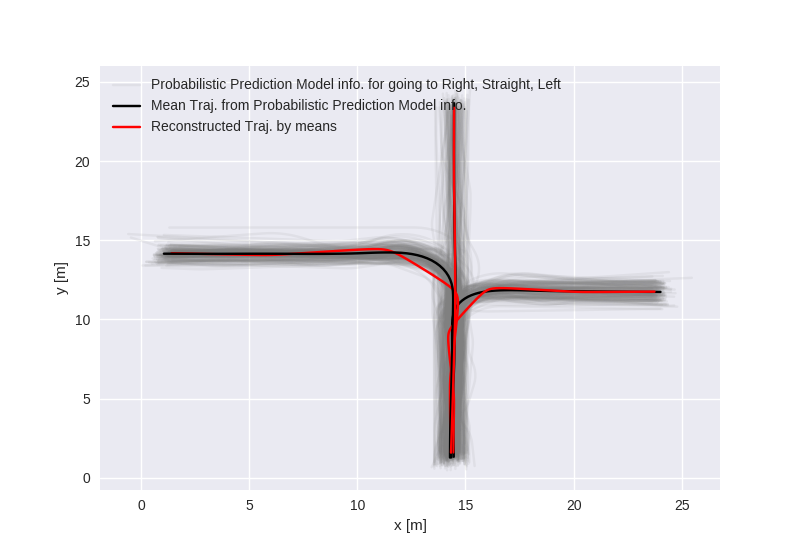
\includegraphics[width=12cm]{img/reconstructedTraj.png}
	\caption{\textcolor{red}{Reconstructed trajectory by means} from probabilistic prediction model. \textcolor{gray}{All pre-recorded demonstrations} and \textbf{mean trajectory}, from probabilistic prediction model}
	\label{fig:ReconstructedTraj}    
\end{figure}

\section{Experiments Using The Real Car Data}

In previous chapters, data collection from a real car and its preparation for work was described. In this section results with real data is described. \\
Due to some technical problems, not all data was good for using, and at the end, we have $15$ trajectories for algorithm learning ($5$ per each movement class) and $3$ trajectories for testing ($1$ per each class). An algorithm training set is shown in Figure~\ref{fig:RealSet}. We will choose trajectory randomly and will make all experiments with that trajectory. Only X intersection will be used for this testing.

\begin{figure}[H]
	\centering  	
	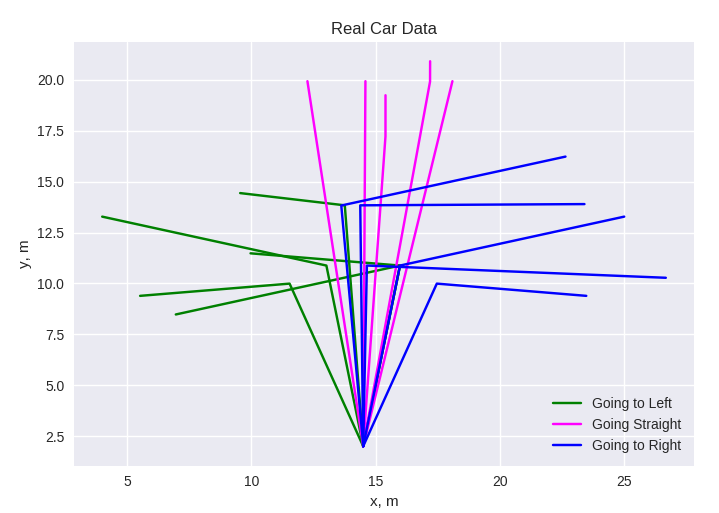
\includegraphics[width=10cm]{img/RealDataSet.png}
	\caption{Trajectories recorded with a real aDDa car. The duration of plotted trajectories is 9 seconds each. Length of trajectories does not match for several reasons: because of  duration unification, car speed and different real trajectory length (one turn was longer, another shorter, etc.)}
	\label{fig:RealSet}    
\end{figure}

For this real car data test, the same algorithm from before was used with different learning and testing data. The first run gave these results: Figure~\ref{fig:RealStraight} and Table \ref{table:realStraight}.

\begin{figure}[H]
	\centering  	
	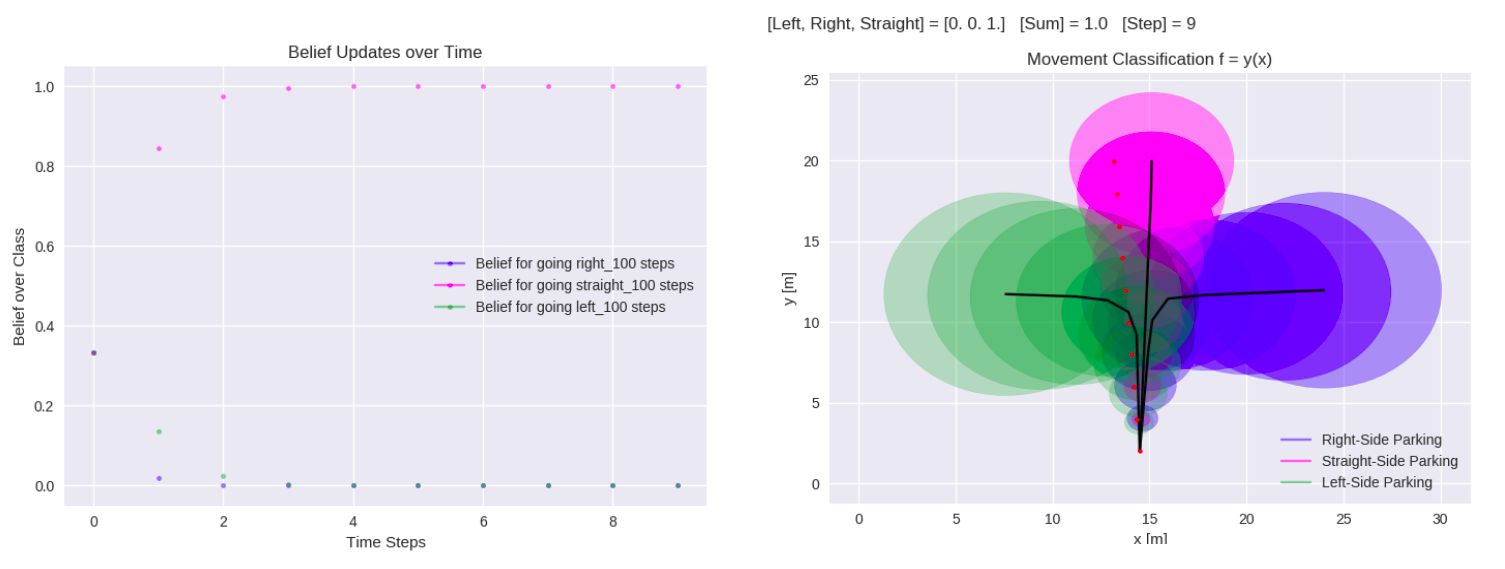
\includegraphics[width=13cm]{img/RealStraight.png}
	\caption{The image on the left side of the figure shows belief updates over time and on the right red dotted line is the tested trajectory, interpolated for $10$ time steps}
	\label{fig:RealStraight}    
\end{figure}

Table \ref{table:realStraight} shows prediction results of each step:

\begin{table}[H]
	\centering
	\begin{tabular}{ |p{1.5cm}||p{1.5cm}|p{1.5cm}|p{1.5cm}|}
		\hline
		\multicolumn{4}{|c|}{Belief that Movement class is ...} \\
		\hline
		Time Step & Right & Left & Straight \\
		\hline
		0 & 0.333 & 0.333 & 0.333 \\
		1 & 0.135 & 0.020 & 0.846 \\
		2 & 0.024 & 0.001 & 0.975 \\
		3 & 0.006 & 0.001 & 0.993 \\
		4 - 7 & 0.001 & 0.0   & 0.999 \\
		8 - 9 & 0.0   & 0.0   & 1.0 \\
		\hline
	\end{tabular}
	\caption{Belief Update Over Time for straight trajectory. Algorithm knew to which direction car is going from the very beginning}
	\label{table:realStraight}
\end{table}

Results of the second run is summarized in Figure~\ref{fig:Realleft} and Table \ref{table:realleft}.

\begin{figure}[H]
	\centering  	
	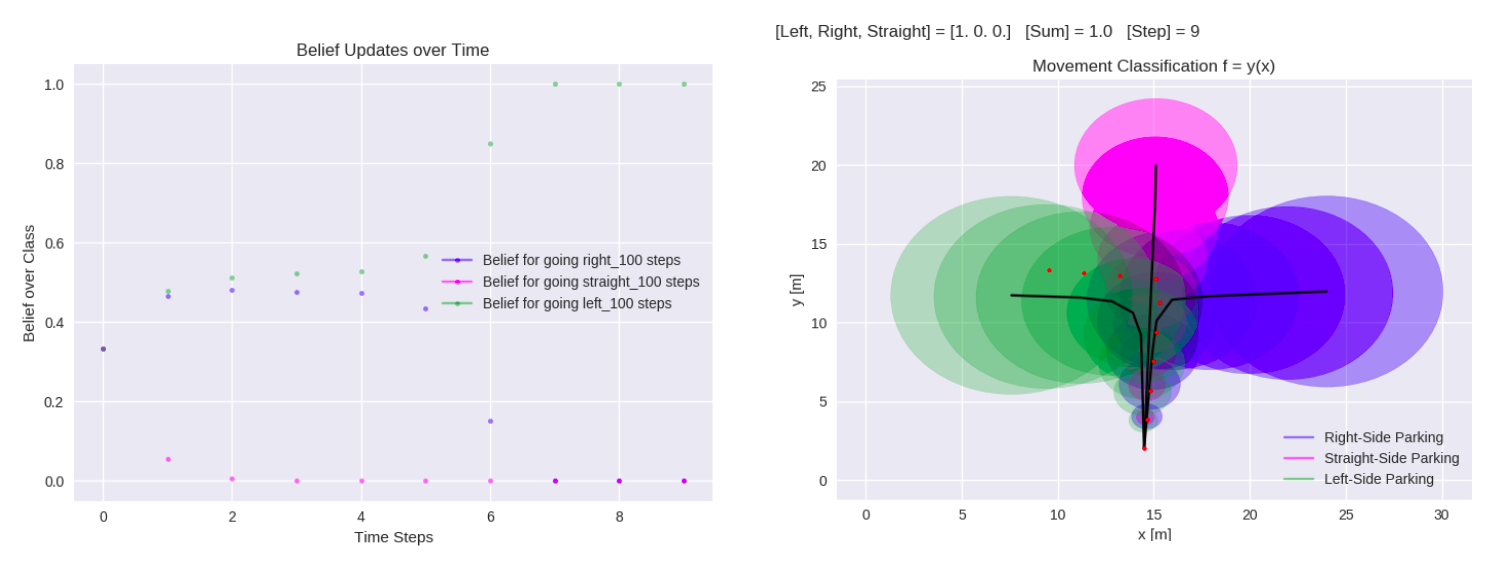
\includegraphics[width=13cm]{img/realLeft.png}
	\caption{The image on the left side of the figure shows belief updates over time and on the right red dotted line is the tested trajectory, interpolated for $10$ time steps}
	\label{fig:Realleft}    
\end{figure}

Table \ref{table:realleft} shows prediction results of each step:

\begin{table}[H]
	\centering
	\begin{tabular}{ |p{1.5cm}||p{1.5cm}|p{1.5cm}|p{1.5cm}|}
		\hline
		\multicolumn{4}{|c|}{Belief that Movement class is ...} \\
		\hline
		Time Step & Right & Left & Straight \\
		\hline
		0 & 0.333 & 0.333 & 0.333 \\
		1 & 0.479 & 0.465 & 0.056 \\
		2 & 0.511 & 0.481 & 0.007 \\
		3 & 0.522 & 0.476 & 0.001 \\
		4 & 0.527 & 0.472 & 0.001 \\
		5 & 0.566 & 0.433 & 0.001 \\
		6 & 0.848 & 0.151 & 0.001 \\
		7 & 0.999 & 0.001 & 0.000 \\
		8 - 9 & 1.0   & 0.0   & 0.0 \\
		\hline
	\end{tabular}
	\caption{Belief Update Over Time for left trajectory. Algorithm was pretty sure to which direction car is going from the very beginning}
	\label{table:realleft}
\end{table}

The last run looked like in Figure~\ref{fig:Realright} and in the Table \ref{table:realright}.

\begin{figure}[H]
	\centering  	
	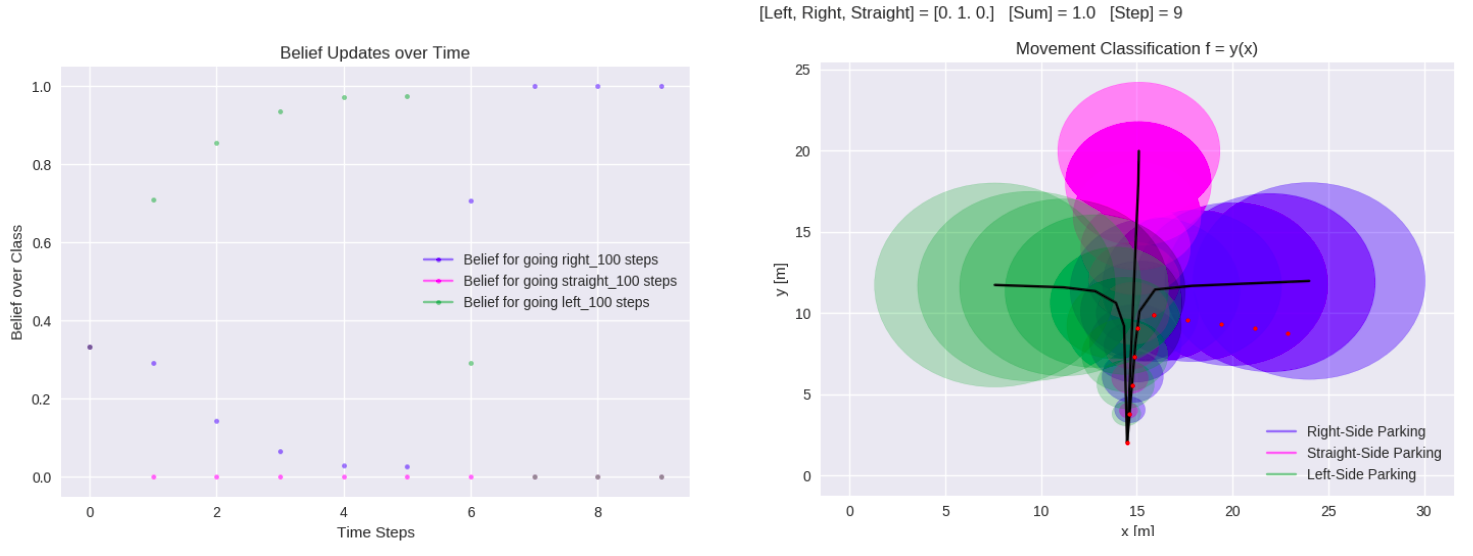
\includegraphics[width=12cm]{img/realRight.png}
	\caption{The image on the left side of the figure shows belief updates over time and on the right red dotted line is the tested trajectory, interpolated for $10$ time steps}
	\label{fig:Realright}    
\end{figure}

Table \ref{table:realright} shows prediction results of each step:

\begin{table}[H]
	\centering
	\begin{tabular}{ |p{1.5cm}||p{1.5cm}|p{1.5cm}|p{1.5cm}|}
		\hline
		\multicolumn{4}{|c|}{Belief that Movement class is ...} \\
		\hline
		Time Step & Right & Left & Straight \\
		\hline
		0 & 0.333 & 0.333 & 0.333 \\
		1 & 0.709 & 0.290 & 0.001 \\
		2 & 0.855 & 0.144 & 0.001 \\
		3 & 0.934 & 0.065 & 0.001 \\
		4 & 0.971 & 0.028 & 0.001 \\
		5 & 0.973 & 0.267 & 0.0 \\
		6 & 0.292 & 0.707 & 0.0 \\
		7 & 0.001 & 0.099 & 0.0 \\
		8 - 9 & 0.0   & 1.0   & 0.0 \\
		\hline
	\end{tabular}
	\caption{Belief Update Over Time for right trajectory. While recognizing right trajectory algorithm thought that car is moving to left direction, but at the end it recognized direction correctly}
	\label{table:realright}
\end{table}

From the results, we can see that the algorithm is working on not only on simulated data but with real information from the car. Results showed that some trajectories were recognized easier than another, unfortunately, due to the lack of testing trajectories, there was no possibility to test different trajectories and to get average results of real trajectories and to understand exactly why this happened. But from experiments with simulated data, we can make an assumption that tested data for right trajectory was not a really smooth one.

\subsection{The Whole Trajectory Reconstruction using \gls{ProMPs}}

The explanation of \gls{ProMPs} is done in the previous chapter. In this set of experiment, we will check how well \gls{ProMPs} method can recreate a trajectory having a number of \gls{RBF} and weights for each function, which was computed from the learning data set. As mentioned in the description chapter of \gls{ProMPs}, it is very important to select the right number of \gls{RBF}. As in the chapter of explanation of the method, the right number of \gls{RBF} we selected by calculating the error of real and reconstructed trajectories (Figure~\ref{fig:error}).

\begin{figure}[H]
	\centering  	
	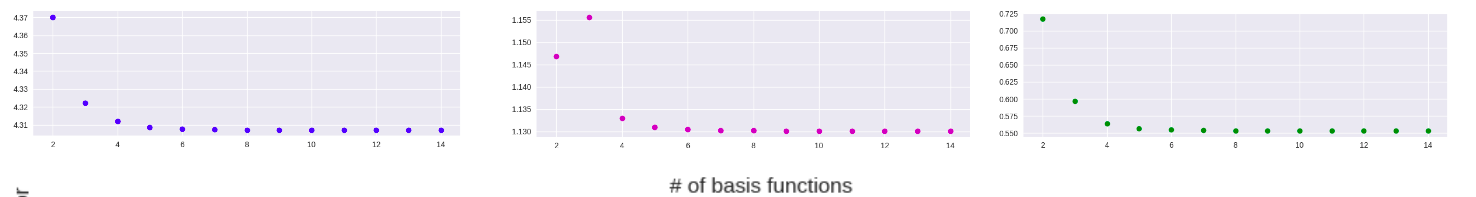
\includegraphics[width=17cm]{img/error.png}
	\caption{Error dependence on number of \gls{RBF}.The right side of the figure shows error for the right movement class, the middle for the straight and the left one - for the left movement class. We can see that the smallest value of trajectory error is when we have $6$ and more \gls{RBF}}
	\label{fig:error}    
\end{figure}

From Figure~\ref{fig:error} we can see that the smallest error value is when we are working with $6$ and more \gls{RBF}, from now we will be working with $6$ \gls{RBF} - there is no need to use bigger number, because it do not do any influence on results, but it very affect computation time.\\

As mentioned before we can calculate weights on the chosen number of training data. We are a reconstructing trajectory in two ways: using the mean of weights for different trajectories and using weights, computed by using only one trajectory. Results are below in Figures ~\ref{fig:recRight}, ~\ref{fig:recLeft} and ~\ref{fig:recStraight}.

\begin{figure}[H]
	\centering  	
	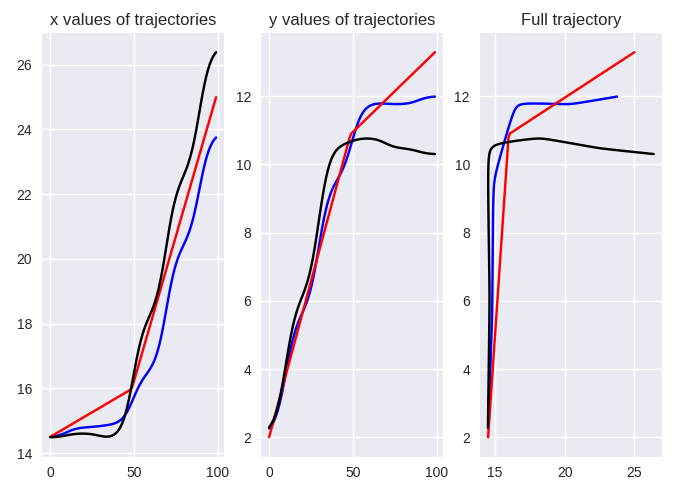
\includegraphics[width=8cm]{img/recRight.png}
	\caption{Reconstructed trajectories. The left side of the figure shows reconstructed x-axis, picture in the middle illustrates reconstructed y-axis, the right side of the figure shows the full reconstructed trajectory. \textcolor{blue}{Blue} line shows reconstructed trajectory, for which reconstruction was used mean of weights of all learning data set, \textbf{black} line shows trajectory reconstructed by weights from one trajectory and \textcolor{red}{red} line shows original trajectory. Movement direction is right}
	\label{fig:recRight}    
\end{figure}

\begin{figure}[H]
	\centering  	
	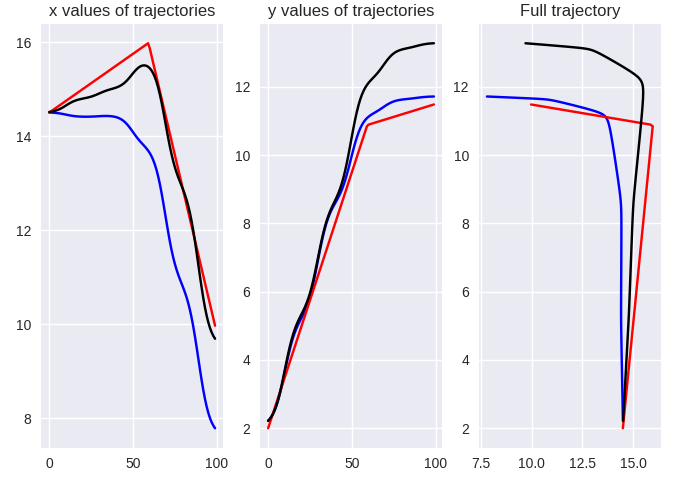
\includegraphics[width=8cm]{img/recLeft.png}
	\caption{Reconstructed trajectories. The left side of the figure shows reconstructed x-axis, picture in the middle illustrates reconstructed y-axis, the right side of the figure shows the full reconstructed trajectory. \textcolor{blue}{Blue} line shows reconstructed trajectory, for which reconstruction was used mean of weights of all learning data set, \textbf{black} line shows trajectory reconstructed by weights from one trajectory and \textcolor{red}{red} line shows original trajectory. Movement direction is left}
	\label{fig:recLeft}    
\end{figure}

\begin{figure}[H]
	\centering  	
	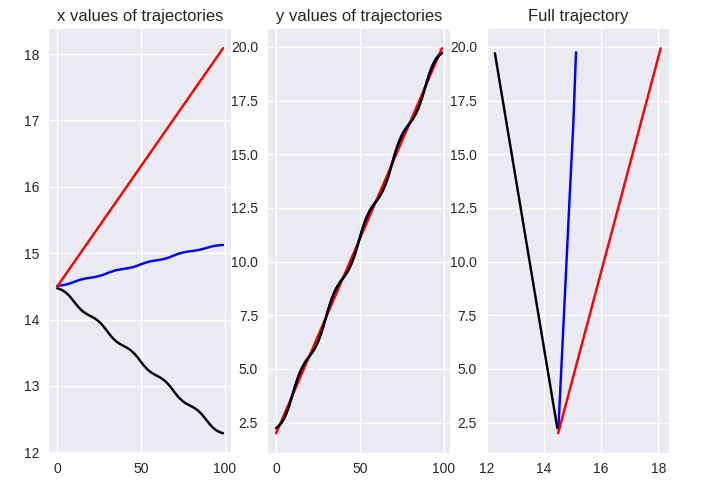
\includegraphics[width=8cm]{img/recStraight.png}
	\caption{Reconstructed trajectories. The left side of the figure shows reconstructed x-axis, picture in the middle illustrates reconstructed y-axis, the right side of the figure shows the full reconstructed trajectory. \textcolor{blue}{Blue} line shows reconstructed trajectory, for which reconstruction was used mean of weights of all learning data set, \textbf{black} line shows trajectory reconstructed by weights from one trajectory and \textcolor{red}{red} line shows original trajectory. Movement direction is straight}
	\label{fig:recStraight}    
\end{figure}

From Figures ~\ref{fig:recRight}, ~\ref{fig:recLeft} and ~\ref{fig:recStraight} we can see that overall trajectory recreated quite close to the real value of the trajectory (if learning data set would be bigger, the recreated trajectory would be even more close) and all trajectories were recreated to the right movement direction.

\section{Future Trajectory Prediction, Using Data, Collected In Real Time}

The difference between the using pre-recorder and real time trajectories is that with pre-recorded trajectories is easier to work, since we know how trajectories looks like, we can unify them and make them to have the same amount of time steps, etc. Pre-recorded testing trajectories is very useful while creating algorithm, it allows easy and quick check of algorithm workflow. Once results are as they are expected to be, the algorithm is used on \gls{ROS} and on its' visualization tool \gls{RViz}. Using these tools driving simulation is happening on the real-time, receiving observed cars' position immediately after it is done - meaning, that all calculations and prediction is making depending must be done quickly and correctly. \\
Before starting to test prediction making algorithm we faced the problem of trajectory length. While working with pre-recorded data, we already had a full trajectory and for testing purposes, we could unify them time-steps wise. This does not work in reality, since we do not know how long driving simulation is going to happen. \\
We solved this problem using minimum distance which theoretically described in the chapter before. After this we tried to predict how full trajectory will look like, using \gls{ProMPs}, which theoretically described also before.

\subsection{Real Time Prediction Making In \gls{ROS} Simulation}

Working with pre-recorded data works only in simulations. In a real-life, it is very important to work with real data, which means having some level of uncertainty. We will provide the results for this experiment with the capture of images from real-time experiments. \\
From the Figure~\ref{fig:inROS}, it is possible to see that real-time prediction is also working. However, in order to avoid delays in calculations, it is better to use a more powerful machine which is responsible for prediction making.

\begin{figure}[H]
	\centering  	
	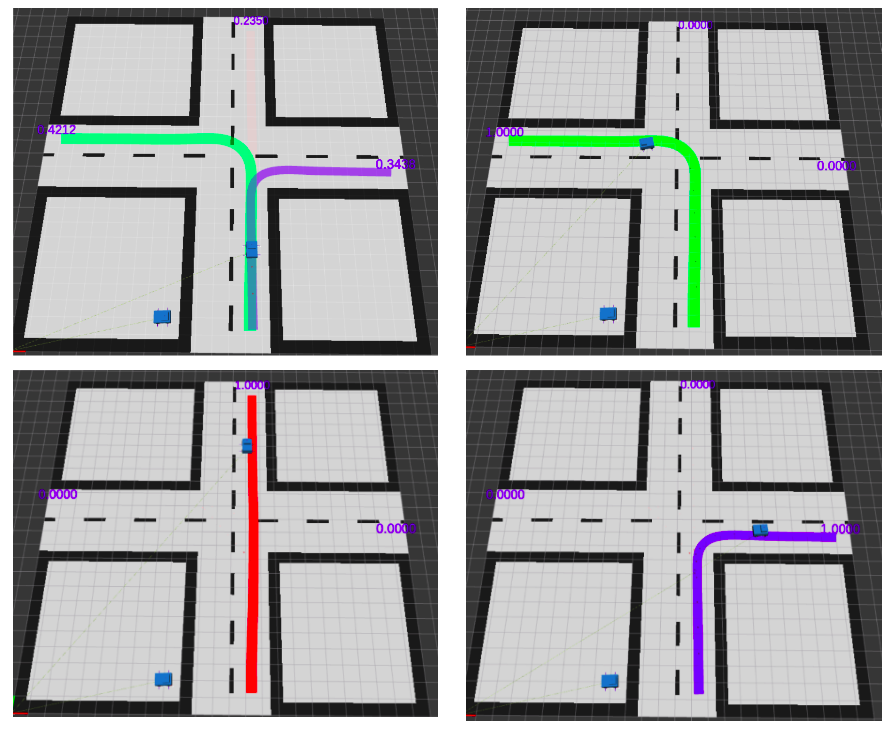
\includegraphics[width=14cm]{img/reallifeExperiments.png}
	\caption{Few captures from proposed probabilistic intention prediction algorithm working on real-time data. The upper left side shows the prediction made while starting to drive. The upper right picture shows results while moving towards the left direction, the bottom left illustrates straight movement class and the bottom right one - right side}
	\label{fig:inROS}    
\end{figure}


% \subsection{Full Trajectory Prediction, using \gls{ProMPs}}


